\documentclass[a4paper,11pt]{article}
\usepackage[utf8]{inputenc}
\usepackage{graphicx}
\usepackage[T2A]{fontenc}
\usepackage[utf8]{inputenc}
\usepackage[english]{babel}
\usepackage{extsizes}
\usepackage{indentfirst}
\usepackage{fancyhdr}
\usepackage{geometry}
\usepackage{amsthm}
\usepackage{amsfonts}
\usepackage{mathtools}
\usepackage{graphicx}
\usepackage{wrapfig}
\usepackage{caption}
\usepackage{amssymb}
\usepackage{booktabs}
\usepackage{dsfont}
\usepackage[toc,page]{appendix}
\usepackage[export]{adjustbox}
\usepackage[percent]{overpic}
\usepackage{pbox}
\usepackage{listings}
\usepackage{xcolor}
\lstset { %
	language=C++,
	backgroundcolor=\color{black!5}, % set backgroundcolor
	basicstyle=\footnotesize,% basic font setting
	keywordstyle=\color[rgb]{0,0,1},
	commentstyle=\color[rgb]{0.026,0.112,0.095},
	stringstyle=\color[rgb]{0.627,0.126,0.941},
	numberstyle=\color[rgb]{0.205, 0.142, 0.73},
	commentstyle=\color{red},
	stringstyle=\color{green}
}

\theoremstyle{plain}
\newtheorem{thm}{Theorem}
\newtheorem{lmm}[thm]{Lemma}
\newtheorem{crlr}[thm]{Corollary}

\theoremstyle{definition}
\newtheorem{defn}[thm]{Definition}
\newtheorem{exmp}[thm]{Example}
\newtheorem{rmrk}[thm]{Remark}
\newtheorem{asmp}[thm]{Assumption}
\newtheorem{prps}[thm]{Proposition}
\newtheorem{cond}[thm]{Conditions}

\graphicspath{{./images/}}

\renewenvironment{proof}{{\scshape Proof:}}{}

\renewcommand{\theenumi}{\roman{enumi}}
\renewcommand{\labelenumi}{(\theenumi)}

\newcommand{\ME}{\mathbb{E}}
\newcommand{\MR}{\mathbb{R}}
\newcommand{\MP}{\mathbb{P}}
\newcommand{\MN}{\mathbb{N}}
\newcommand{\MZ}{\mathbb{Z}}
\newcommand{\Var}{\operatorname{Var}}
\newcommand{\Cov}{\operatorname{Cov}}
\newcommand{\diag}{\operatorname{diag}}
\newcommand{\tr}{\operatorname{tr}}
\newcommand{\convdistr}{\xrightarrow{\mathcal{L}}}
\newcommand{\convprob}{\xrightarrow{\MP}}
\newcommand{\define}[1]{\textit{\textbf{#1}}}
\bgroup
\def\arraystretch{2}%  1 is the default, change whatever you need
%opening
\title{RandLib documentation}
\author{Aleksandr Samarin}

\begin{document}
	
	\maketitle
	\tableofcontents
	
	\pagebreak
	\part{General information}
	\section{Calculation of sample moments}
	We use extension of Welford's method from Knuth. For every $n$-th element $x$ we have
	\[
	\begin{aligned}
	\delta &= x - m_1, \\
	m_1' &= m_1 +  \frac{\delta}{n}, \\
	m_2' &= m_2 +  \delta^2 \frac{n-1}{n}, \\
	m_3' &= m_3 + \delta^3 \frac{(n-1)(n-2)}{n^2} - 3\delta \frac{m_2}{n}, \\
	m_4' &= m_4 +  \delta^4 \frac{(n-1)(n^2-3n+3)}{n^3}+6\delta^2 \frac{m_2}{n^2}-4\delta\frac{m_3}{n}.
	\end{aligned}
	\]
	Then $ m_1'$, $\frac{m_2}{n}$, $\operatorname{Skew}(X) = \frac{\sqrt{n}m_3'}{m_2'^{3/2}}$ and $\operatorname{Kurt}(X) = \frac{nm_4'}{m_2'^2}$ (we return excess kurtosis). 
	
	\pagebreak
	\part{Continuous univariate distributions}
	\section{Beta distribution}
		\begin{figure}[!htb]\centering
			\begin{minipage}{0.55\textwidth}
				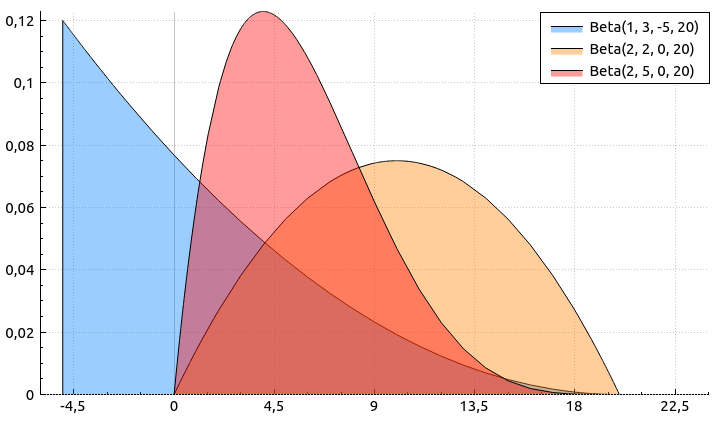
\includegraphics[width=\linewidth, right]{beta_pdf}
				\captionsetup{labelformat=empty}
				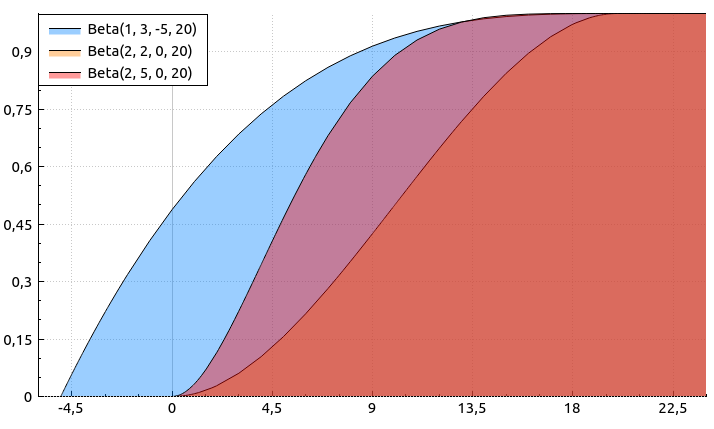
\includegraphics[width=\linewidth, right]{beta_cdf}
				\captionsetup{labelformat=empty}
			\end{minipage}
			\begin{minipage}{0.4\textwidth}
		\begin{tabular}{| r | l |}
			\hline
			Notation & \pbox{\linewidth}{$ X \sim \mathcal{B}(\alpha, \beta, a, b)$ \\ $X \sim \mathcal{B}(\alpha, \beta)$ with $a=0, b=1$} \\
			\hline
			Parameters & $\alpha, \beta > 0$, $a, b \in \MR$ \\
			\hline
			Domain & $x \in [a, b]$  \\
			\hline
			$f(x)$ & $\frac{y^{\alpha - 1}(1 - y)^{\beta - 1}}{(b-a)B(\alpha, \beta)}$ with $y = \frac{x - a}{b - a}$ \\
			\hline
			$F(x)$ & $I_{y}(\alpha, \beta)$ for $y = \frac{x - a}{b - a}$\\
			\hline
			$\ME[X]$ & $a + (b-a)\frac{\alpha}{\alpha + \beta}$ \\
			\hline
			$\Var(X)$ & $(b-a)^2\frac{ \alpha \beta}{(\alpha + \beta)^2 (\alpha + \beta + 1)}$ \\
			\hline
			Median & Searched numerically \\
			\hline
			Mode & $a + (b-a)\frac{\alpha - 1}{\alpha + \beta - 2}$ for $\alpha, \beta > 1$. \\
			\hline
			$\phi(t)$ & Calculated numerically \\
			\hline
		\end{tabular}
	\end{minipage}
	\end{figure}
	
	\paragraph{Search of the median.}
	In general, the value of median is unkwnown and searched numerically with initial value:
	\[
	m \approx a + (b-a)\frac{\alpha - \frac{1}{3} }{ \alpha + \beta - \frac{2}{3} }
	\]
	for $\alpha, \beta \geq 1$.	However, there are analytical solutions for some particular values:
	\begin{itemize}
		\item $m = \frac{a + b}{2}$, for $\alpha = \beta$,
		\item $m = a + (b-a)(1 - 2^{-\frac{1}{\beta}})$, for $\alpha = 1$,
		\item $m = a+(b-a)2^{-\frac{1}{\alpha}}$, for $\beta = 1$.
	\end{itemize}
	
	\paragraph{Calculation of characteristic function.}
	For $\alpha, \beta \geq 1$ we use numerical integration by definition
	\[
	\phi(t) = \int_a^b \cos(tx) f(x) dx + i \int_{a}^{b} \sin(tx) f(x) dx.
	\]
	For shape parameters $<1$, $f(x)$ has singularity points at $0$ or $1$ or both of them, and numerical integration is impossible. Then we use the following technique: firstly, we can show that
	\[
	\phi(t|a, b) = \ME[e^{it(a + (b-a)X)}] = e^{ita} \phi(z|0, 1)
	\]
	with $z = (b-a)t$. Hence, w.l.o.g. we can consider standard case $a=0$, $b=1$. Then
	\[
	\begin{aligned}
	\Re(\phi(z)) & = \frac{1}{B(\alpha, \beta)} \int_{0}^{1} \cos(zx) x^{\alpha-1} (1-x)^{\beta-1} dx\\
	& = \frac{1}{B(\alpha, \beta)} \int_{0}^{1} (\cos(zx)-1) x^{\alpha-1} (1-x)^{\beta-1} dx + 1 \\
	& = \frac{1}{B(\alpha, \beta)} \int_{0}^{1} \frac{(\cos(zx)-1) x^{\alpha-1} - (\cos(z)-1)}{(1-x)^{1-\beta}}  dx + 1 + \frac{\cos(z) - 1}{bB(\alpha, \beta)}.
	\end{aligned}
	\]
	The integrand now doesn't have any singularities, neither for $\alpha<1$, nor for $\beta < 1$. Analogously we transform the imaginary part:
	\[
	\begin{aligned}
	\Im(\phi(z)) & = \frac{1}{B(\alpha, \beta)} \int_{0}^{1} \sin(zx) x^{\alpha-1} (1-x)^{\beta-1} dx\\
	& = \frac{1}{B(\alpha, \beta)} \int_{0}^{1} \frac{\sin(zx) x^{\alpha-1} - \sin(z)}{(1-x)^{1-\beta}}  dx + \frac{\sin(z)}{bB(\alpha, \beta)}.
	\end{aligned}
	\]
	
	\paragraph{Estimation of shapes with known support.} Assume that $a=0$, $b=1$ and we have a sample $X = (X_1, \dots, X_n)$. Then a log-likelihood function is
	\begin{equation} \label{Beta log-likelihood}
	\begin{aligned}
	\ln \mathcal{L} (\alpha, \beta | X) &= \sum_{i=1}^{n} \ln f(X_i; \alpha, \beta) \\
	& = (\alpha - 1) \sum_{i=1}^{n} \ln X_i + (\beta - 1) \sum_{i=1}^{n}\ln (1-X_i) - n \ln B(\alpha, \beta).
	\end{aligned}  
	\end{equation}
	Differentiating with respect to the shapes, we obtain
	\[
	\frac{\partial \ln \mathcal{L}(\alpha, \beta | X)}{\partial \alpha} = \sum_{i=1}^{n} \ln X_i + n(\psi(\alpha + \beta) - \psi(\alpha)),
	 \]
	\[
	\frac{\partial \ln \mathcal{L}(\alpha, \beta | X)}{\partial \beta} = \sum_{i=1}^{n} \ln (1-X_i) + n(\psi(\alpha + \beta) - \psi(\beta)).
	\]
	Differentiating again we get the Hessian matrix:
	\[
	\operatorname{H}(\ln\mathcal{L}(\alpha,\beta|X)) = n \cdot \begin{pmatrix}
	\psi_1(\alpha+\beta)-\psi_1(\alpha) & \psi_1(\alpha+\beta) \\
	\psi_1(\alpha+\beta) & \psi_1(\alpha+\beta)-\psi_1(\beta)
	\end{pmatrix}.
	\]
	Then we can find the estimators numerically, using Newton's procedure. The initial values of estimators are found via method of moments:
	\[
	\hat{\alpha}_0 = \overline{X}_n \Bigg( \frac{\overline{X}_n(1-\overline{X}_n)}{\hat{s}_n^2} - 1 \Bigg),
	\]
	\[
	\hat{\beta}_0 = (1-\overline{X}_n) \Bigg( \frac{\overline{X}_n(1-\overline{X}_n)}{\hat{s}_n^2} - 1 \Bigg).
	\]
	These values are applicable only if $\hat{s}_n^2 < \overline{X}_n(1-\overline{X}_n)$. If this condition is not satisfied, we set $\hat{\alpha}_0 = \hat{\beta}_0 = 0.001$.\\
	In the general case, when $a \neq 0$ or $b \neq 1$, we use the following transformation:
	\[ Y_i = \frac{X_i - a}{b - a} \]
	and estimate parameters, using sample $Y$.
	
	\subsection{Arcsine distribution}
	Notation:
	\[
	X \sim \operatorname{Arcsine}(\alpha).
	\]
	Relation to Beta distribution: \[ X \sim \mathcal{B}(1-\alpha, \alpha, a, b). \]
	\paragraph{Estimation of shape.} For Arcsine distribution log-likelihood function \eqref{Beta log-likelihood} turns into
	\[
	\ln \mathcal{L} (\alpha | X) = -\alpha \sum_{i=1}^{n} \ln X_i + (\alpha - 1) \sum_{i=1}^{n}\ln (1-X_i) - n \ln B(1-\alpha, \alpha).
	\]
	Taking the derivative with respect to $\alpha$ we get
	\[ 
	\frac{\partial \ln\mathcal{L}(\alpha | X)}{\partial \alpha} = \sum_{i=1}^{n} \ln \frac{1-X_i}{X_i} + n\pi \cot(\pi \alpha).
	\]
	Therefore, maximum-likelihood function is
	\[ \hat{\alpha} = -\frac{1}{\pi} \operatorname{atan}\Bigg(\frac{n\pi}{\sum_{i=1}^{n} \ln \frac{1-X_i}{X_i}}\Bigg). \]
	If $\hat{\alpha}$ is negative, we add $1$, because $\frac{\operatorname{atan}}{\pi} \in (-0.5, 0.5)$, while $\alpha \in (0, 1)$.
	
	\subsection{Balding-Nichols distribution}
	Notation: \[ X \sim \operatorname{Balding-Nichols}(p, F) \] with $p, F \in (0, 1)$.
	Relation to Beta distribution: \[ X \sim \mathcal{B}(pF', (1 - p)F') \] with $F' = (1 - F) / F$.
	
	\subsection{Uniform distribution}
	\begin{figure}[!htb]\centering
		\begin{minipage}{0.55\textwidth}
			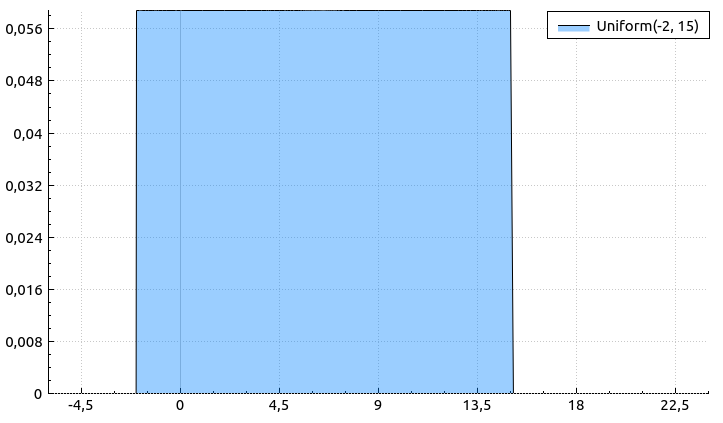
\includegraphics[width=\linewidth, right]{uniform_pdf}
			\captionsetup{labelformat=empty}
			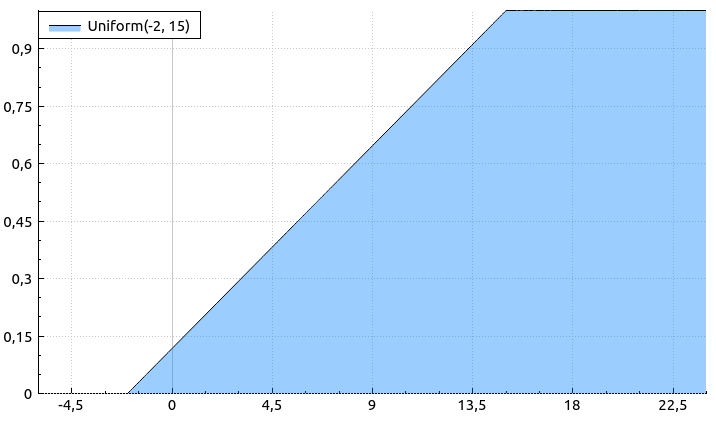
\includegraphics[width=\linewidth, right]{uniform_cdf}
			\captionsetup{labelformat=empty}
		\end{minipage}
		\begin{minipage}{0.4\textwidth}
			\begin{tabular}{| r | l |}
				\hline
				Notation & $ X \sim \mathcal{U}(a, b)$ \\
				\hline
				Parameters & $a, b \in \MR$ \\
				\hline
				Domain & $x \in [a, b]$  \\
				\hline
				$f(x)$ & $\frac{1}{b - a}$ \\
				\hline
				$F(x)$ & $\frac{x - a}{b - a}$\\
				\hline
				$\ME[X]$ & $ \frac{a+b}{2}$ \\
				\hline
				$\Var(X)$ & $\frac{(b-a)^2}{12}$ \\
				\hline
				Median & $\frac{a+b}{2}$ \\
				\hline
				Mode & doesn't exist \\
				\hline
				$\phi(t)$ & $ \frac{e^{itb}-e^{ita}}{it(b-a)} $ \\
				\hline
			\end{tabular}
		\end{minipage}
	\end{figure}
	
	Relation to Beta distribution: \[X \sim \mathcal{B}(1, 1, a, b). \]
	\paragraph{Estimation of support.}
	\subparagraph{Frequentist inference.} Likelihood function is
	\[
	\mathcal{L}(a, b | X) = \frac{1}{(b-a)^n} \mathbf{1}_{ \{ X_i \in [a, b] \ \forall i = 1, \dots, n \} }.
	\]
	Therefore, $\mathcal{L}(a, b | X)$ is the largest for $\hat{b} = X_{(n)}$ and $\hat{a} = X_{(1)}$. However, using the fact that $X_{(k)} \sim B(k, n+1-k, a, b)$, these are biased estimators:
	\[ \ME[X_{(1)}] = \frac{an + b}{n+1} \quad \text{and} \quad \ME[X_{(n)}] = \frac{a + bn}{n+1}.  \]
	To get unbiased estimators we make the transformations:
	\[ \tilde{a} = \frac{nX_{(1)} - X_{(n)} }{n-1} \quad \text{and} \quad  \tilde{b} = \frac{nX_{(n)} - X_{(1)} }{n-1}. \]
	Then we get
	\[ 
	\ME[\tilde{a}] = \frac{n\ME[X_{(1)}] - \ME[X_{(n)}]}{n-1} = \frac{n(an+b)-(a+bn)}{n^2-1} = a.
	\]
	Analogously, $\ME[\tilde{b}] = b$.
	\subparagraph{Bayesian inference.} Let us say, we try to estimate $\theta = b-a$ with known $a$. We set the prior distribution $\theta \sim \operatorname{Pareto}(\alpha, \sigma)$:
	\[
	h(\theta|\alpha, \sigma) = \frac{\alpha \sigma^\alpha}{\theta^{\alpha + 1}} \mathbf{1}_{\{\theta \geq \sigma\}}.
	\]
	The density of posterior distribution is
	\[
	f(\theta|X) \propto \frac{\alpha \sigma^\alpha}{\theta^{\alpha+n+1}} \mathbf{1}_{\{\theta \geq \max(\sigma, X_{(n)}-a) \}} \sim \operatorname{Pareto}(\alpha + n, \max(\sigma, X_{(n)}-a) ).
	\]
	Hence, Bayesian estimator is
	\[  
	\ME[\theta|X] = \frac{\alpha + n}{\alpha + n - 1}\max(\sigma, X_{(n)}-a)
	\]
	and MAP estimator is
	\[
	\theta_{MAP} = \max(\sigma, X_{(n)}-a).
	\]
	
	\pagebreak
	\section{Beta-prime distribution}
		\begin{figure}[!htb]\centering
		\begin{minipage}{0.55\textwidth}
			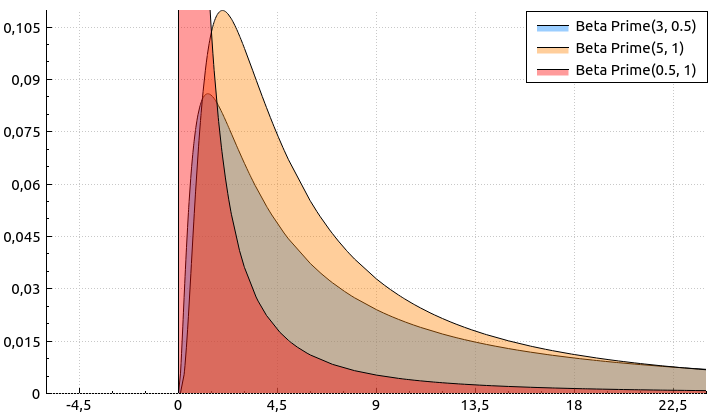
\includegraphics[width=\linewidth, right]{beta_prime_pdf}
			\captionsetup{labelformat=empty}
			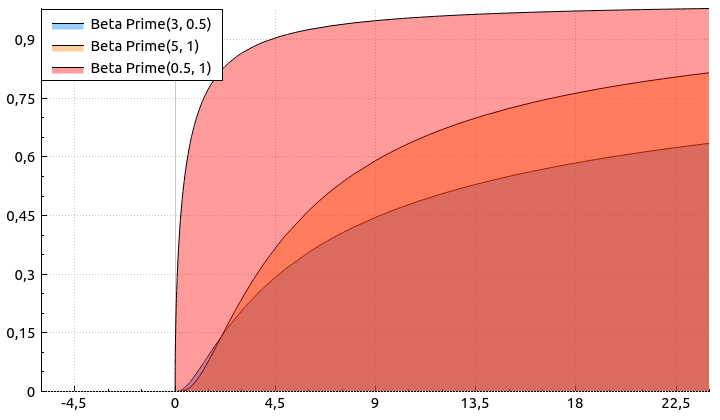
\includegraphics[width=\linewidth, right]{beta_prime_cdf}
			\captionsetup{labelformat=empty}
		\end{minipage}
		\begin{minipage}{0.4\textwidth}
			\begin{tabular}{| r | l |}
				\hline
				Notation & $X \sim \mathcal{B}'(\alpha, \beta)$ \\
				\hline
				Parameters & $\alpha, \beta > 0$ \\
				\hline
				Domain & $x \in \MR^+$  \\
				\hline
				$f(x)$ & $\frac{x^{\alpha - 1}(1 + x)^{-\alpha - \beta}}{B(\alpha, \beta)}$ \\
				\hline
				$F(x)$ & $I_{\frac{x}{1+x}}(\alpha, \beta)$\\
				\hline
				$\ME[X]$ & $ \frac{\alpha}{\beta - 1}\mathbf{1}_{\{\beta > 1 \} } + \infty \mathbf{1}_{\{\beta \leq 1\} } $ \\
				\hline
				$\Var(X)$ & $\frac{ \alpha (\alpha +\beta - 1) }{ (\beta-2)(\beta-1)^2 }$, if $\beta > 1$ \\
				\hline
				Median & Searched numerically \\
				\hline
				Mode & $\max\big( \frac{\alpha-1}{\beta+1}, 0 \big)$. \\
				\hline
				$\phi(t)$ & Calculated numerically \\
				\hline
			\end{tabular}
		\end{minipage}
	\end{figure}
	Relation to other distributions:
	\[\frac{X}{1+X} \sim \mathcal{B}(\alpha, \beta),\]
	\[
	\frac{\beta}{\alpha}X \sim F(2\alpha, 2\beta ).
	\]
	
	\paragraph{Search of the median.} For $\alpha = \beta$ we have $m=1$. Otherwise, we use the relation
	$m = \frac{m'}{1-m'},$
	where $m'$ is the median of beta-distribution $\mathcal{B}(\alpha, \beta)$.
	
	\paragraph{Calculation of characteristic function.} For $\alpha \geq 1$ one can use numerical integration from section %todo add section
	For $\alpha < 1$ we have $\lim_{x \rightarrow 0} f(x) \rightarrow \infty$ and $\int_{0}^{\infty} \cos(tx)f(x) dx$ is impossible to compute directly. Then we split the integral:
	\[
	\int_{0}^{\infty} \cos(tx)f(x) dx = \int_{0}^{\infty}(\cos(tx)-1) f(x) dx + 1.
	\]
	The limit of the integrand for $x \rightarrow 0$ is $0$ now, regardless of the value of the shape $\alpha$.
	
	\paragraph{Estimation of shapes.} Using relationship with Beta distribution we transform the sample:
	\[ Y_i = \frac{X_i}{1+X_i}, \quad 1 \leq i \leq N, \]
	and run estimation for beta-distributed $Y$.

	\pagebreak
	\section{Exponentially-modified Gaussian distribution}
	\begin{figure}[!htb]\centering
		\begin{minipage}{0.55\textwidth}
			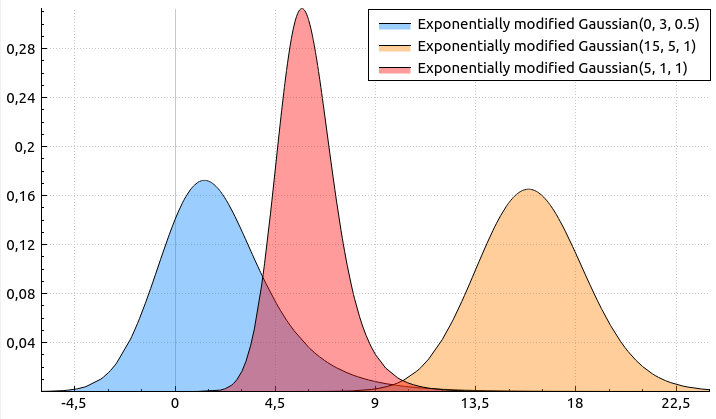
\includegraphics[width=\linewidth, right]{emg_pdf}
			\captionsetup{labelformat=empty}
			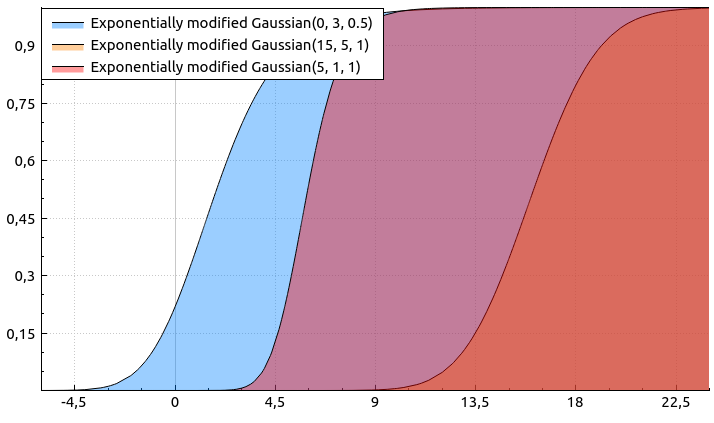
\includegraphics[width=\linewidth, right]{emg_cdf}
			\captionsetup{labelformat=empty}
		\end{minipage}
		\begin{minipage}{0.4\textwidth}
		\begin{tabular}{| r | l |}
			\hline
			Notation & $X \sim \operatorname{EMG}(\mu, \sigma, \lambda)$ \\
			\hline
			Parameters & $\mu \in \MR, \sigma > 0, \lambda > 0$ \\
			\hline
			Domain & $x \in \MR$  \\
			\hline
			$f(x)$ & $ \frac{\lambda}{2} e^{\frac{\lambda}{2}(2\mu + \lambda \sigma^2 - 2x)} \operatorname{erfc} \Big( \frac{\mu + \lambda \sigma^2 - x}{\sqrt{2\sigma^2}} \Big) $ \\
			\hline
			$F(x)$ &\pbox{\linewidth}{$ \Phi(u,0,v)-e^{ -u + \frac{v^2}{2} +\log \Phi(u, v^2, v) }, $\\ where  $\Phi(x, \mu, \sigma)$ is Gaussian CDF, \\ $u=\lambda(x-\mu),$ \\ $v=\lambda \sigma$. } \\
			\hline
			$\ME[X]$ & $ \mu + 1 / \lambda$ \\
			\hline
			$\Var(X)$ & $\sigma^2 + 1/\lambda^2$ \\
			\hline
			Median & Searched numerically \\
			\hline
			Mode & Searched numerically \\
			\hline
			$\phi(t)$ & $ \big(1-\frac{it}{\lambda} \big)^{-1}  \exp \big(i\mu t - \frac{1}{2} \sigma^2 t^2 \big) $ \\
			\hline
		\end{tabular}
	\end{minipage}
\end{figure}
    Relation to other distribution: if $X \sim \mathcal{N}(\mu, \sigma^2)$ and $Y \sim \operatorname{Exp}(\lambda)$, then $X + Y \sim \operatorname{EMG}(\mu, \sigma, \lambda)$.
	
	
	\pagebreak
	\section{F-distribution}
		\begin{center}
			\begin{tabular}{| r | l |}
				\hline
				Notation & $X \sim \operatorname{F}(d_1, d_2)$ \\
				\hline
				Parameters & $d_1, d_2 > 0$ \\
				\hline
				Domain & $x \in \MR^+$  \\
				\hline
				$f(x)$ & $\frac{\sqrt{\frac{(d_1 x)^{d_1} {d_2}^{d_2} }{(d_1x+d_2)^{d_1+d_2}}}}{x B\Big(\frac{d_1}{2},\frac{d_2}{2}\Big)}  $ \\
				\hline
				$F(x)$ & $ I_{\frac{d_1x}{d_1x+d_2}}\Big(\frac{d_1}{2},\frac{d_2}{2}\Big) $\\
				\hline
				$\ME[X]$ & $ \frac{d_2}{d_2-2}$ for $ d_2 > 2 $ \\
				\hline
				$\Var(X)$ & $\frac{2d_2^2(d_1+d_2-2)}{d_1(d_2-2)^2(d_2-4)}$ for $d_2 > 4$ \\
				\hline
				Median & Searched numerically \\
				\hline
				Mode & $\max\Big(\frac{d_2(d_1-2)}{d_1(d_1+2)}, 0\Big)$ \\
				\hline
				$\phi(t)$ & Calculated numerically \\
				\hline
			\end{tabular}
		\end{center}
		Relation to other distributions:
		\[
		\frac{d_1X}{d_2 + d_1X} \sim \mathcal{B}\bigg(\frac{d_1}{2}, \frac{d_2}{2} \bigg),
		\]
		\[
		\frac{d_1}{d_2}X \sim \mathcal{B}'\bigg(\frac{d_1}{2}, \frac{d_2}{2} \bigg).
		\]
		
		
	\pagebreak
	\section{Gamma distribution}
	\begin{figure}[!htb]\centering
		\begin{minipage}{0.55\textwidth}
			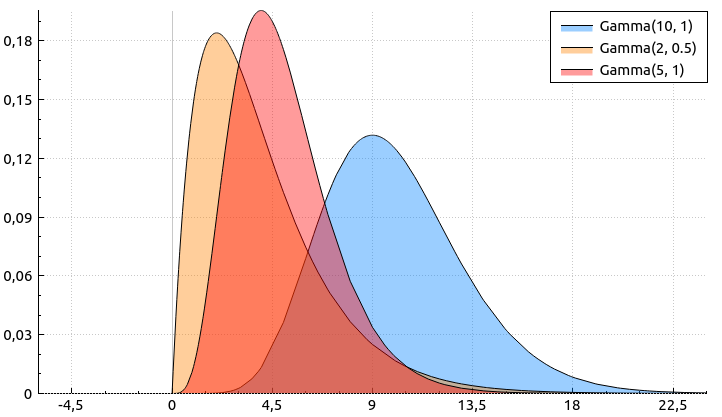
\includegraphics[width=\linewidth, right]{gamma_pdf}
			\captionsetup{labelformat=empty}
			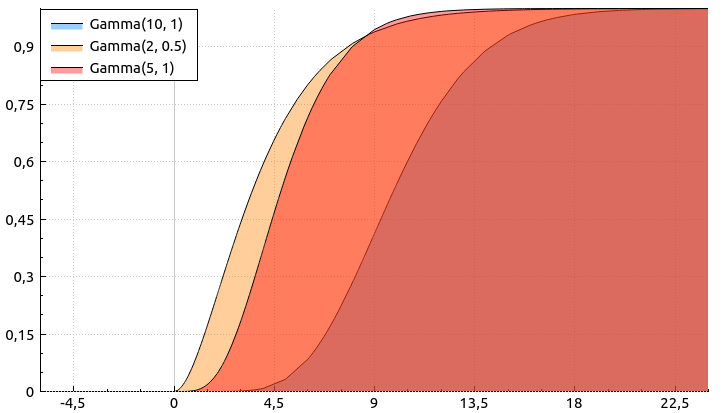
\includegraphics[width=\linewidth, right]{gamma_cdf}
			\captionsetup{labelformat=empty}
		\end{minipage}
		\begin{minipage}{0.4\textwidth}
			\begin{tabular}{| r | l |}
				\hline
				Notation & $X \sim \Gamma(\alpha, \beta)$ \\
				\hline
				Parameters & $\alpha > 0, \beta > 0$ \\
				\hline
				Domain & $x \in \MR^+$  \\
				\hline
				$f(x)$ & $\frac{\beta^\alpha}{\Gamma(\alpha)} x^{\alpha-1}e^{-\beta x}  $ \\
				\hline
				$F(x)$ & $P(\alpha, \beta x) $\\
				\hline
				$\ME[X]$ & $ \frac{\alpha}{\beta}$ \\
				\hline
				$\Var(X)$ & $\frac{\alpha}{\beta^2}$ \\
				\hline
				Median & Searched numerically \\
				\hline
				Mode & $\max\big(\frac{\alpha - 1}{\beta}, 0\big)$ \\
				\hline
				$\phi(t)$ & $ \Big( 1-\frac{it}{\beta} \Big)^{-\alpha}$ \\
				\hline
			\end{tabular}
		\end{minipage}
	\end{figure}
	
	\paragraph{Estimation of parameters.}
	\subparagraph{Frequentist inference.} Log-likelihood function:
	\[
	\ln \mathcal{L}(\alpha, \beta|X) =  n \alpha \ln \beta - n \ln \Gamma(\alpha) + (\alpha - 1) \sum_{i=1}^{n} \ln X_i - \beta \sum_{i=1}^{n} X_i.
	\]
	Derivatives:
	\[
	\frac{\partial \ln \mathcal{L}(\alpha, \beta | X) }{\partial \alpha} = n \ln \beta - n \psi (\alpha) + \sum_{i=1}^{n} \ln X_i,
	\]
	\[
	\frac{\partial \ln \mathcal{L}(\alpha, \beta | X) }{\partial \beta} = \frac{n \alpha}{\beta} - \sum_{i=1}^{n} X_i.
	\]
	While the solution for the second equation is analytic:
	\[
	\hat{\beta} = \frac{\alpha}{\overline{X}_n},
	\]
	the first equation is solved numerically, using second derivative:
	\[
	\frac{\partial^2 \ln \mathcal{L}(\alpha, \beta | X) }{\partial \alpha^2} = - n \psi_1 (\alpha),
	\]
	or if $\beta$ is unknown:
	\[
	\frac{\partial^2 \ln \mathcal{L}(\alpha, \beta | X) }{\partial \alpha^2} = - n \psi_1 (\alpha) + \frac{n}{\alpha},
	\]
	Moreover, the maximum-likelihood estimation of rate $\beta$ is biased. Unbiased estimator would be
	\[
	\tilde{\beta} = \frac{\alpha}{\overline{X}_n} \Big(1 - \frac{1}{n}\Big).
	\]
	\subparagraph{Bayesian inference.} We suppose that prior distribution of rate $\beta$ is $\Gamma(\kappa, \gamma)$:
	\[
	h(\beta) = \frac{\gamma^\kappa}{\Gamma(\kappa)} \beta^{\kappa-1}e^{-\gamma \beta}.
	\]
	Then
	\[
	f(\beta | X) \propto \beta^{\alpha n} e^{-\beta \sum_{i=1}^{n} X_i } \cdot \beta^{\kappa-1}e^{-\gamma \beta} \sim \operatorname{\Gamma}\Big(\alpha n + \kappa, \gamma +\sum_{i=1}^{n} X_i \Big).
	\]
	Therefore, Bayesian estimator is
	\[
	\ME[\beta|X] = \frac{\alpha n + \kappa}{\gamma +\sum_{i=1}^{n} X_i},
	\]
	and MAP estimator is
	\[
	\beta_{MAP} = \frac{\alpha n + \kappa - 1}{\gamma +\sum_{i=1}^{n} X_i}.
	\]
	
	\paragraph{Exponential family parameterization}
	Logarithm of probability mass function:
	\[
	\log \MP(X = x) = \alpha \log \beta - \log \Gamma(\alpha) + (\alpha - 1) \log x - \beta x.
	\]
	Therefore, sufficient statistics $T(x) = (\log x, x)^T$, natural parameters $\theta = (\alpha-1, -\beta)$, log-normalizer $F(\theta) = \log \Gamma (\theta_1 + 1) - (\theta_1 + 1) \log (-\theta_2)$, carrier measure $k(x) = 0$. Gradient of log-normalizer is $\nabla F(\theta) = \big(\psi(\theta_1 + 1) - \log(-\theta_2), -\frac{\theta_1+1}{\theta_2} \big)^T$ We conclude that adjusted cross-entropy is
	\[
	\begin{aligned}
	H_F(\theta_q \| \theta_p) &= F(\theta_q) - \langle \theta_q, \nabla F(\theta_p) \rangle \\
	&= \log \Gamma ({\theta_q}_1 + 1) - ({\theta_q}_1 + 1) \log (-{\theta_q}_2) - {\theta_q}_1 (\psi({\theta_p}_1 + 1) - \log(-{\theta_p}_2)) + \frac{{\theta_q}_2 ({\theta_p}_1 + 1)}{{\theta_p}_2}.
	\end{aligned}
	\]
	Adjusted entropy is
	\[
	\begin{aligned}
	H_F(\theta) &= \log \Gamma ({\theta}_1 + 1) - \log (-{\theta}_2) - {\theta}_1 \psi({\theta}_1 + 1) + {\theta}_1 + 1 \\
	& = \log \Gamma (\alpha) - \log \beta - (\alpha - 1) \cdot \psi (\alpha) + \alpha.
	\end{aligned}
	\]
	And Kullback-Leibler divergence:
	\[
	\begin{aligned}
	\operatorname{KL}(p \| q) &= H_F(\theta_q \| \theta_p) - H_F(\theta_p) \\
	&= \log \frac{\Gamma (\alpha_q)}{\Gamma (\alpha_p)} + \alpha_q \log \frac{\beta_p}{\beta_q} + (\alpha_p - \alpha_q) \psi(\alpha_p) + \alpha_p \bigg(\frac{\beta_q}{\beta_p} - 1\bigg)
	\end{aligned}
	\]
	
	\subsection{Chi-squared distribution}
	Notation:
	\[
	X \sim \chi_k^2.
	\]
	Relation to Gamma distribution:
	\[
	X \sim \Gamma\bigg( \frac{k}{2}, \frac{1}{2} \bigg).
	\]
	Kullback-Leibler divergence:
	\[
	\operatorname{KL}(p \| q) = \log \frac{\Gamma(k_q/2)}{\Gamma(k_p/2)} + \frac{1}{2}(k_p - k_q) \psi(k_p / 2).
	\]
	Relation to other distributions: if $X_1, \dots, X_k ~ \sim \mathcal{N}(0, 1)$, then $\sum_{i=1}^{k}X_i \sim \chi_k^2$.
	
	\subsection{Erlang distribution}
	Notation:
	\[
	X \sim \operatorname{Erlang}(k, \beta).
	\]
	The only difference between Gamma and Erlang distributions is that latter takes an integer number $k$ as a shape parameter.
	
	\subsection{Exponential distribution}
	\begin{figure}[!htb]\centering
		\begin{minipage}{0.55\textwidth}
			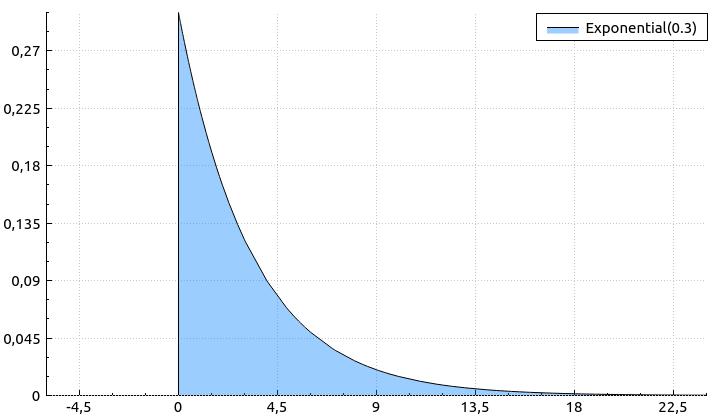
\includegraphics[width=\linewidth, right]{exponential_pdf}
			\captionsetup{labelformat=empty}
			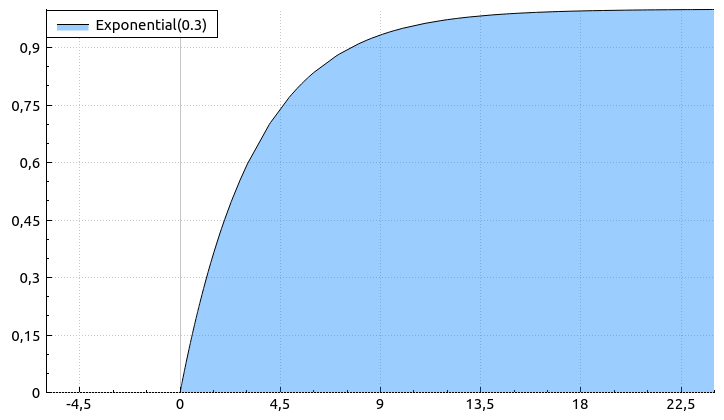
\includegraphics[width=\linewidth, right]{exponential_cdf}
			\captionsetup{labelformat=empty}
		\end{minipage}
		\begin{minipage}{0.4\textwidth}
		\begin{tabular}{| r | l |}
			\hline
			Notation & $X \sim \operatorname{Exp}(\lambda)$ \\
			\hline
			Parameters & $\lambda > 0$ \\
			\hline
			Domain & $x \in \MR^+$  \\
			\hline
			$f(x)$ & $\lambda e^{-\lambda x}  $ \\
			\hline
			$F(x)$ & $1-e^{-\lambda x} $\\
			\hline
			$\ME[X]$ & $ \frac{1}{\lambda}$ \\
			\hline
			$\Var(X)$ & $\frac{1}{\lambda^2}$ \\
			\hline
			Median & $\frac{\ln(2)}{\lambda}$ \\
			\hline
			Mode & $0$ \\
			\hline
			$\phi(t)$ & $ \frac{\lambda}{\lambda-it}$ \\
			\hline
		\end{tabular}
		\end{minipage}
	\end{figure}

	Relation to Gamma distribution:
	\[X \sim \Gamma(1, \lambda).\]
	Hence, estimation of parameter $\lambda$ is the particular case of estimation of rate $\beta$ for Gamma distribution. \\
	Adjusted cross-entropy:
	\[
	H_F(\lambda_q \| \lambda_p) = \frac{\lambda_q}{\lambda_p}-\log \lambda_q. 
	\]
	Thus adjusted entropy is
	\[
	H_F(\lambda) = 1 - \log \lambda
	\]
	and Kullback-Leibler divergence:
	\[
	\operatorname{KL}(p \| q) = \log \frac{\lambda_p}{\lambda_q} + \frac{\lambda_q}{\lambda_p} - 1.
	\]
	
	\pagebreak
	\section{Geometric Stable distribution}
	\begin{figure}[!htb]\centering
		\begin{minipage}{0.55\textwidth}
			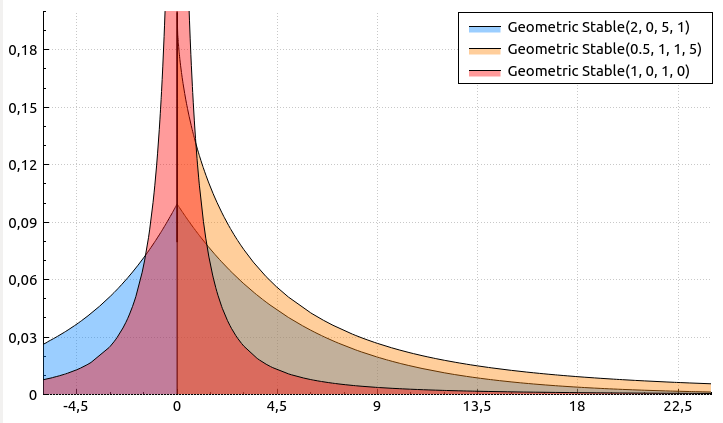
\includegraphics[width=\linewidth, right]{geometric_stable_pdf}
			\captionsetup{labelformat=empty}
			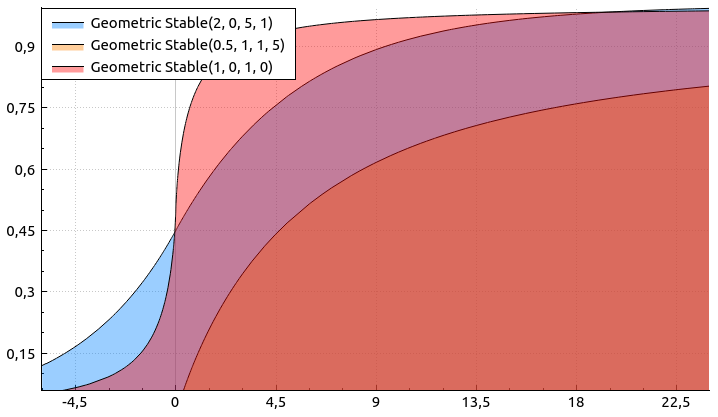
\includegraphics[width=\linewidth, right]{geometric_stable_cdf}
			\captionsetup{labelformat=empty}
		\end{minipage}
		\begin{minipage}{0.4\textwidth}
			\begin{tabular}{| r | l |}
				\hline
				Notation & $X \sim \operatorname{GS}_\alpha(\beta, \gamma, \mu)$ \\
				\hline
				Parameters & \pbox{\linewidth}{$\alpha \in (0, 2], \beta \in [-1, 1],$\\ $\gamma > 0, \mu \in \MR $} \\
				\hline
				Domain & $x \in ...$  \\
				\hline
				$f(x)$ & Calculated numerically \\
				\hline
				$F(x)$ & Calculated numerically \\
				\hline
				$\ME[X]$ & $ k + \lambda$ \\
				\hline
				$\Var(X)$ & $2(k+2\lambda)$ \\
				\hline
				Median & Searched numerically \\
				\hline
				Mode & Searched numerically \\
				\hline
				$\phi(t)$ & $ ...$ \\
				\hline
			\end{tabular}
		\end{minipage}
	\end{figure}
	
	\subsection{Asymmetric Laplace distribution}

	\subsection{Laplace distribution}
	
	\pagebreak
	\section{Kolmogorov-Smirnov distribution}
	\pagebreak
	\section{Logistic distribution}
	\pagebreak
	\section{Log-normal distribution}
	\pagebreak
	\section{Marchenko-Pastur distribution}
	\begin{center}
		\begin{tabular}{| r | l |}
			\hline
			Notation & $X \sim \mathcal{MP}(\lambda, \sigma^2)$ \\
			\hline
			Parameters & $\lambda, \sigma^2 > 0$ \\
			\hline
			Domain & 
			\pbox{\linewidth}{$x \in [\sigma^2 a, \sigma^2 b]$, if  $\lambda < 1$, \\  $ x \in [\sigma^2 a, \sigma^2 b] \cup \{0\} $, otherwise, \\ where $a=(1-\sqrt{\lambda})^2$ and $b=(1+\sqrt{\lambda})^2$} \\
			\hline
			$f(x)$ & ...  \\
			\hline
			$F(x)$ & ... \\
			\hline
			$\ME[X]$ & $ \sigma^2 $ \\
			\hline
			$\Var(X)$ & $\sigma^4 \lambda $ \\
			\hline
			Median & $0$ if $\lambda > 2$, otherwise searched numerically \\
			\hline
			Mode & \pbox{\linewidth}{$\frac{\sigma^2(\lambda - 1)^2}{\lambda+1}$, if  $\lambda < 1$, \\  $ 0 $, otherwise } \\
			\hline
			$\phi(t)$ & Calculated numerically \\
			\hline
		\end{tabular}
	\end{center}
	
	\paragraph{Calculation of characteristic function.}
	For $\lambda > 1$ we use numerical integration by definition
	\[
	\phi(t) = \int_{\sigma^2 a}^{\sigma^2 b} \cos(tx) f(x) dx + i \int_{\sigma^2 a}^{\sigma^2 b}  \sin(tx) f(x) dx.
	\]
	For $\lambda = 1$ we split the integrand for real part by $(\cos(tx) - 1) f(x)$ and $f(x)$:
	\[ \Re(\phi(t)) =  \int_{\sigma^2 a}^{\sigma^2 b} (\cos(tx)-1) f(x) dx + 1.\]
	And for $\lambda < 1$ we calculate integral at point $0$ separately:
	\[
	\begin{aligned}
	\phi(t) & = \int_{ \{0\} \cup [\sigma^2 a, \sigma^2 b]} \cos(tx) f(x) dx + i \int_{ \{0\} \cup [\sigma^2 a, \sigma^2 b]} \sin(tx) f(x) dx  \\ 
	& = 1-\frac{1}{\lambda} + \int_{\sigma^2 a}^{\sigma^2 b} \cos(tx) f(x) dx + i \int_{\sigma^2 a}^{\sigma^2 b}  \sin(tx) f(x) dx.
	\end{aligned}
	\]
	
	
	\pagebreak
	\section{Nakagami distribution}
	\begin{figure}[!htb]\centering
		\begin{minipage}{0.55\textwidth}
			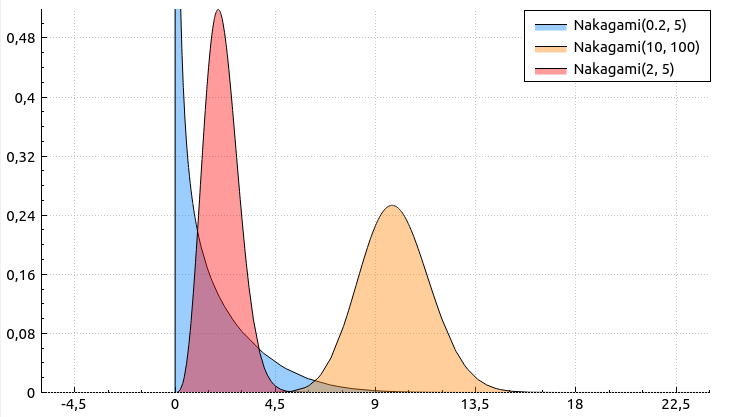
\includegraphics[width=\linewidth, right]{nakagami_pdf}
			\captionsetup{labelformat=empty}
			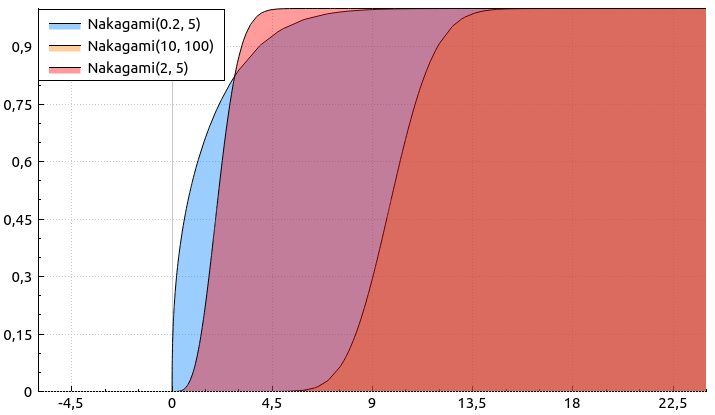
\includegraphics[width=\linewidth, right]{nakagami_cdf}
			\captionsetup{labelformat=empty}
		\end{minipage}
		\begin{minipage}{0.4\textwidth}
			\begin{tabular}{| r | l |}
				\hline
				Notation & $X \sim \operatorname{Nakagami}(\mu, \omega)$ \\
				\hline
				Parameters & $\mu, \omega > 0$ \\
				\hline
				Domain & $x \in \MR^+$  \\
				\hline
				$f(x)$ & $ \frac{2\mu^\mu}{\Gamma(\mu) \omega^\mu} x^{2\mu - 1} e^{-\frac{\mu}{\omega}x^2}   $ \\
				\hline
				$F(x)$ & $P(\mu, \mu x^2/\omega) $\\
				\hline
				$\ME[X]$ & $ \frac{\Gamma(\mu + 1/2)}{\Gamma(\mu)} \sqrt{\frac{\omega}{\mu}}  $ \\
				\hline
				$\Var(X)$ & $\omega - (\ME[X])^2$ \\
				\hline
				Median & Searched numerically \\
				\hline
				Mode & $ \max \bigg( \sqrt{\frac{(2\mu-1)\omega}{2\mu}}, 0\bigg)$ \\
				\hline
				$\phi(t)$ & Calculated numerically \\
				\hline
			\end{tabular}
		\end{minipage}
	\end{figure}
	\paragraph{Calculation of characteristic function.} For $\mu < 1$ $\lim_{x \rightarrow 0}f(x) \rightarrow \infty$. Then we use the following transformation for real part of characteristic function:
	\[
	\begin{aligned}
	\Re(\phi(t)) & = \int_{0}^{\infty} \cos(tx) f(x) dx \\ &= \int_{0}^{\infty} (\cos(tx)-1) f(x) + 1
	\end{aligned}
	\]
	
	Relation to other distributions: if $Y \sim \Gamma\big(\mu, \mu/\omega\big)$, then
	\[
	X \sim \operatorname{Nakagami}(\mu, \omega).
	\]
	
	\subsection{Chi distribution}
	Notation:
	\[
	X \sim \chi_k
	\]
	Relation to Nakagami distribution:
	\[
	X \sim \operatorname{Nakagami}\big(k/2, k\big).
	\]
	
	\subsection{Maxwell-Bolzmann distribution}
	Notation:
	\[
	X \sim \operatorname{MB}(\sigma)
	\]
	Relation to Nakagami distribution:
	\[
	X \sim \operatorname{Nakagami}\big(3/2, \sigma^2 \big).
	\]
	
	\subsection{Rayleigh distribution}
	Notation:
	\[
	X \sim \operatorname{Rayleigh}(\sigma)
	\]
	Relation to Nakagami distribution:
	\[
	X \sim \operatorname{Nakagami}\big(1, 2\sigma^2\big).
	\]
	\paragraph{Estimation of scale.}
	...%TODO: add estimation for whole Nakagami (look wiki)
	
	\pagebreak
	\section{Noncentral Chi-Squared distribution}
	\begin{figure}[!htb]\centering
	\begin{minipage}{0.55\textwidth}
		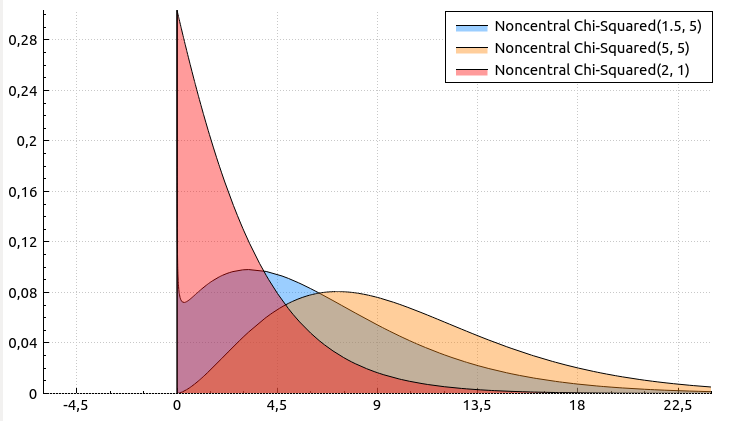
\includegraphics[width=\linewidth, right]{noncentral_chi-squared_pdf}
		\captionsetup{labelformat=empty}
		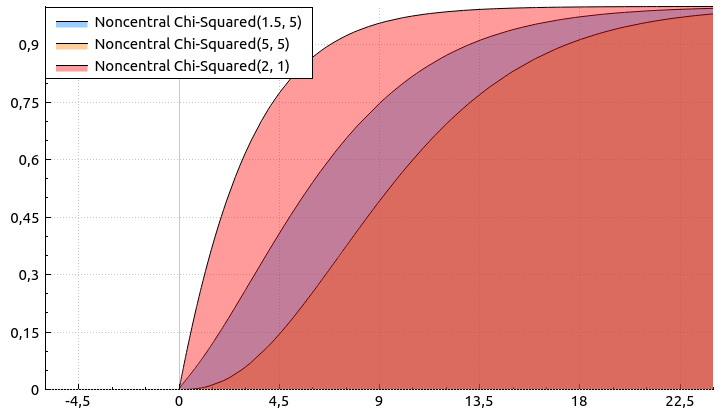
\includegraphics[width=\linewidth, right]{noncentral_chi-squared_cdf}
		\captionsetup{labelformat=empty}
	\end{minipage}
	\begin{minipage}{0.4\textwidth}
		\begin{tabular}{| r | l |}
			\hline
			Notation & $X \sim \chi'^2_k(\lambda)$ \\
			\hline
			Parameters & $k > 0, \lambda > 0$ \\
			\hline
			Domain & $x \in \MR^+$  \\
			\hline
			$f(x)$ & $ \frac{1}{2} e^{-\frac{x+\lambda}{2}}  \Big( \frac{x}{\lambda} \Big)^{\frac{k-2}{4}} I_{\frac{k}{2}-1}(\sqrt{\lambda x})   $ \\
			\hline
			$F(x)$ & $\operatorname{MarcumP}_{\frac{k}{2}}(\frac{\lambda}{2}, \frac{x}{2}) $\\
			\hline
			$\ME[X]$ & $ k + \lambda$ \\
			\hline
			$\Var(X)$ & $2(k+2\lambda)$ \\
			\hline
			Median & Searched numerically\\
			\hline
			Mode & \pbox{\linewidth}{Searched numerically for $k > 2$, \\ $0$, otherwise}  \\
			\hline
			$\phi(t)$ & $ \frac{\exp{\frac{it\lambda}{1-2it}}}{(1-2it)^{k/2}}$ \\
			\hline
		\end{tabular}
	\end{minipage}
    \end{figure}
    Relation to other distributions: 
    \begin{itemize}
    	\item Let $X_1, \dots, X_k$ be independent with $X_i \sim \mathcal{N}(\mu_i, 1)$, $i = 1, \dots, k$. Then
    	\[
    	\sum_{i=1}^{k}X_i^2 \sim \chi'^2_k\big(\sum_{i=1}^{k}\mu_i^2\big).
    	\]
    	\item If $\lambda = 0$, then $X \sim \chi^2_k$.
    	\item If $J \sim \operatorname{Po}(\lambda)$, then $\chi^2_{k+2J} \sim \chi'^2_k(\lambda)$.
    \end{itemize}
    

\pagebreak
\section{Pareto distribution}
\begin{figure}[!htb]\centering
	\begin{minipage}{0.55\textwidth}
		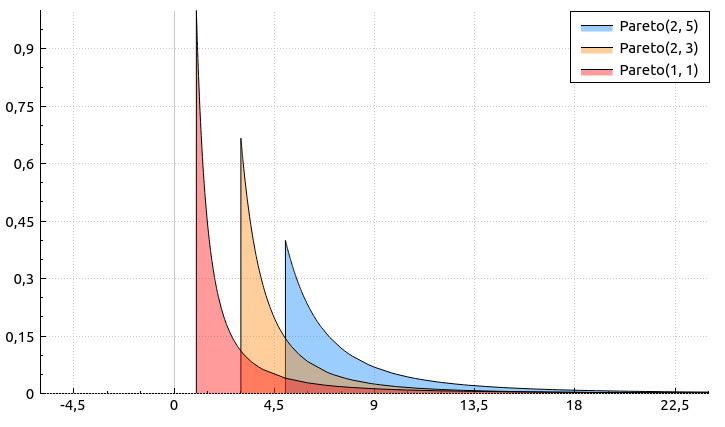
\includegraphics[width=\linewidth, right]{pareto_pdf}
		\captionsetup{labelformat=empty}
		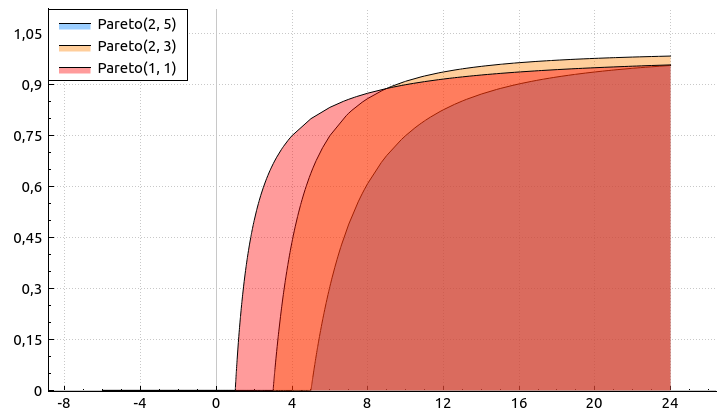
\includegraphics[width=\linewidth, right]{pareto_cdf}
		\captionsetup{labelformat=empty}
	\end{minipage}
	\begin{minipage}{0.4\textwidth}
		\begin{tabular}{| r | l |}
			\hline
			Notation & $X \sim \operatorname{Pareto}(\alpha, \sigma)$ \\
			\hline
			Parameters & $\alpha,  \sigma > 0 $ \\
			\hline
			Domain & $x \geq \sigma$  \\
			\hline
			$f(x)$ & $ \frac{\alpha \sigma^\alpha}{x^{\alpha+1}}  $ \\
			\hline
			$F(x)$ & $ 1-\big( \frac{\sigma}{x} \big)^\alpha $ \\
			\hline
			$\ME[X]$ & \pbox{\linewidth}{$ \frac{\alpha\sigma}{\alpha-1}$ for $\alpha > 1$, \\ $\infty$ otherwise} \\
			\hline
			$\Var(X)$ & \pbox{\linewidth}{$\frac{\sigma^2 \alpha}{(\alpha-1)^2(\alpha-2)}$ for $\alpha > 2$, \\ $\infty$ otherwise } \\
			\hline
			Median & $\sigma 2^{1/\alpha}$ \\
			\hline
			Mode & $\sigma$ \\
			\hline
			$\phi(t)$ & Calculated numerically \\
			\hline
		\end{tabular}
	\end{minipage}
\end{figure}

\paragraph{Estimation of parameters.}
\subparagraph{Frequentist inference.} Log-likelihood function is
\[
\ln \mathcal{L}(\alpha, \sigma | X) = n \ln \alpha + n \alpha \ln \sigma - (\alpha + 1) \sum_{i=1}^{n} \ln X_i.
\]
We assume that $\sigma \leq X_{(1)}$, otherwise sample $X$ couldn't have been generated from such distribution. It is obvious, that $\ln \mathcal{L}(\alpha, \sigma | X)$ is an increasing function in terms of $\sigma$, therefore $\hat{\sigma} = X_{(1)}$ is an optimal estimator.
Let's take derivative with respect to $\alpha$:
\[
\frac{\partial \ln \mathcal{L}(\alpha, \sigma | X) }{\partial \alpha} = \frac{n}{\alpha} + n \ln \sigma - \sum_{i=1}^{n} \ln X_i.
\]
From this we conclude that the maximum-likelihood estimator of shape is
\[
\hat{\alpha} = \frac{1}{ \frac{1}{n} (\sum_{i=1}^{n} \ln X_i) - \ln \hat{\sigma} }.
\]
It is known that $\hat{\sigma} \sim \operatorname{Pareto}(n\alpha, \sigma)$ and $\hat{\alpha} \sim \operatorname{Inv-\Gamma}(n-1, n\alpha)$ and they are independent. Then
\[ \ME[\hat{\sigma}] = \frac{ \sigma}{1-\frac{1}{n \alpha}}\]
and
\[ \ME[\hat{\alpha}] = \frac{n\alpha}{n-2}. \]
Therefore, in order to get unbiased estimators we need to make the following transformations:
\[ \tilde{\alpha} = \frac{n-2}{n}\hat{\alpha} \quad \text{and} \quad \tilde{\sigma} = \hat{\sigma} \bigg(1 - \frac{1}{(n-1)\hat{\alpha}}\bigg). \]
Note that if we estimate parameters separately, then $\hat{\alpha} \sim \operatorname{Inv-\Gamma}(n, n\alpha)$ and transformations are different.

\subparagraph{Bayesian inference.} We now assume that $\sigma$ is known and prior distribution of $\alpha$ is $\Gamma(\kappa, \beta)$:
\[
h(\alpha) = \frac{\beta^\kappa}{\Gamma(\kappa)} \alpha^{\kappa-1}e^{-\beta \alpha}.
\]
The density of posterior distribution is
\[
f(\alpha | X) \propto \prod_{i=1}^n \frac{\sigma^\alpha}{{X_i}^{\alpha-1}} \cdot \alpha^{\kappa+n-1}e^{-\beta \alpha} \propto \alpha^{\kappa+n-1} e^{ -(\beta + \sum_{i=1}^n \ln (X_i/\sigma))\alpha }.
\]
Therefore, $\alpha |X \sim \Gamma(\kappa + n, \beta +\sum_{i=1}^n \ln (X_i/\sigma))$ and Bayesian estimator is
\[ \ME[\alpha | X] = \frac{\kappa + n}{ \beta +\sum_{i=1}^n \ln (X_i/\sigma) }. \]
MAP estimator is
\[ \alpha_{MAP} = \frac{\kappa + n-1}{ \beta +\sum_{i=1}^n \ln (X_i/\sigma) }. \]
\textit{Note on fitting scale with Bayes:} let it be vice versa, $\alpha$ is known while $\sigma$ is not. Then we say that a priori $\sigma \sim \operatorname{Pareto}(\kappa, \theta)$:
\[
h(\sigma) = \frac{\kappa\theta^\kappa}{\sigma^{\kappa+1}}.
\]
Then posterior distribution is:
\[
f(\sigma|X) \propto \prod_{i=1}^n \frac{1}{{X_i}^{\alpha-1}} \cdot \sigma^{\alpha n - \kappa - 1} \mathbf{1}_{ \{ \theta < \sigma < X_{(1)}\} } \sim \operatorname{Bounded-Pareto}(\kappa-\alpha n, \theta, X_{(1)}).
\]
This imposes the following additional constraints on the prior hyperparameters: $\kappa > \alpha n$ and $\theta < X_{(1)}$. Bayesian estimator:
\[
\ME[\sigma|X] = \frac{\theta^{\alpha'}}{1-\Big(\frac{\theta}{X_{(1)}}\Big)^{\alpha'}} \cdot \Big(\frac{\alpha'}{\alpha'-1}\Big)\cdot \bigg( \frac{1}{\theta^{\alpha'}} -\frac{1}{X_{(1)}^{\alpha'}} \bigg)
\]
with $\alpha'=\kappa - \alpha n$.
MAP estimator is just
\[
\sigma_{MAP} = \theta.
\]
However, Bounded-Pareto distribution is not yet supported in RandLib.

	
	\pagebreak
	\section{Planck distribution}
	
	\begin{figure}[!htb]\centering
		\begin{minipage}{0.55\textwidth}
			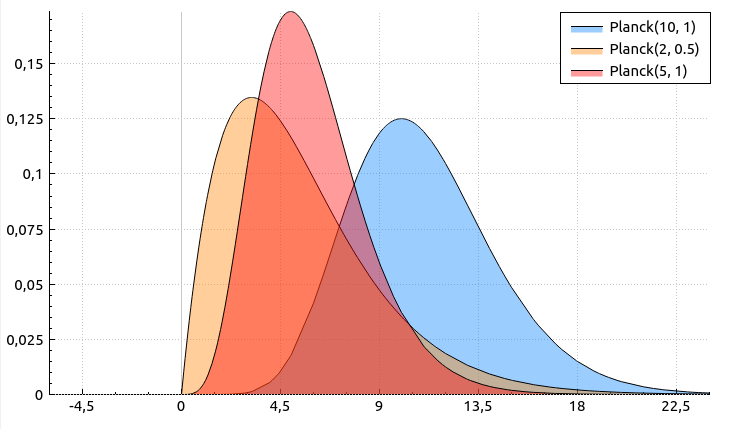
\includegraphics[width=\linewidth, right]{planck_pdf}
			\captionsetup{labelformat=empty}
			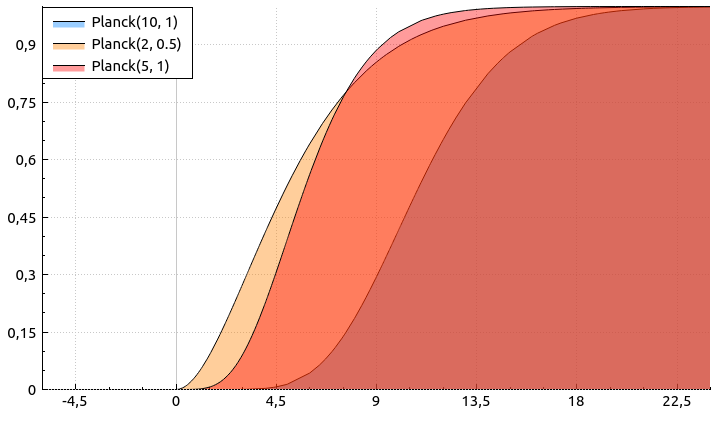
\includegraphics[width=\linewidth, right]{planck_cdf}
			\captionsetup{labelformat=empty}
		\end{minipage}
		\begin{minipage}{0.4\textwidth}
		\begin{tabular}{| r | l |}
			\hline
			Notation & $X \sim \operatorname{Planck}(a, b)$ \\
			\hline
			Parameters & $a, b > 0$ \\
			\hline
			Domain & $ x \in \MR^+$  \\
			\hline
			$f(x)$ & $\frac{b^{a+1}}{\Gamma(a+1)\zeta(a+1)} \cdot \frac{x ^ a}{e^{bx} - 1}$ \\
			\hline
			$F(x)$ & Calculated numerically \\
			\hline
			$\ME[X]$ & $ \frac{(a+1)\zeta(a+2)}{b \zeta(a+1)}$ \\
			\hline
			$\Var(X)$ & $\frac{(a+1)(a+2)\zeta(a+3)}{b^2 \zeta(a+1)}  - (\ME[X])^2$ \\
			\hline
			Median & Searched numerically \\
			\hline
			Mode & $\frac{W_0(-a e^{-a}) + a}{b}$, if $a > 1$, otherwise $0$ \\
			\hline
			$\phi(t)$ & Calculated numerically \\
			\hline
		\end{tabular}
	\end{minipage}
    \end{figure}
    \paragraph{Calculation of cumulative distribution function.} For $a \geq 1$ $F(x)$ can be calculated by straightforward numerical integration:
    \[
    F(x) = \frac{b^{a+1}}{\Gamma(a+1)\zeta(a+1)} \int_{0}^{x} \frac{t ^ a}{e^{bt} - 1} dt.
    \]
    Note that for $\alpha < 1$ integrand has a singularity point at $t=0$. In such case we define
    \[
    h(t) = \frac{b^{a+2}t ^ {a+1} }{\Gamma(a+1)\zeta(a+1)} \cdot \bigg( \frac{1}{e^{bt} -  1}-\frac{1}{bt}\bigg)
    \]
    and then
    \[
    F(x) = \int_{0}^{x}  h(t) dt + \frac{(bx)^{a}}{a\Gamma(a+1)\zeta(a+1)}.
    \]
	
	\paragraph{Calculation of characteristic function.} The idea of calculations for $a < 1$ is near the same. We split the real part of $\phi(t)$ into $3$ different integrals:
	\[
	\Re(\phi(t)) = \int_{0}^{1} \cos(tx) h(x) dx + \int_{1}^{\infty} \cos(tx) f(x{\tiny }) dx + \frac{b^{a}}{a\Gamma(a+1)\zeta(a+1)} \bigg(\cos(t) + t\int_{0}^{1} \sin(tx)x^a dx \bigg).
	\]
	All the indegrands now have no singularity points.
	
	\pagebreak
	\section{Stable distribution}
	\begin{figure}[!htb]\centering
		\begin{minipage}{0.55\textwidth}
			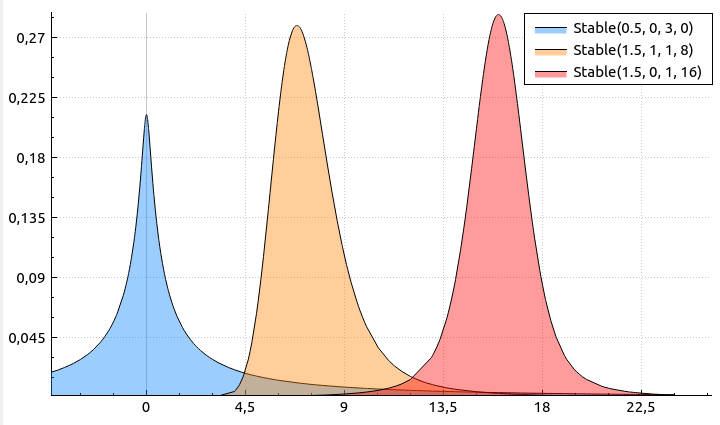
\includegraphics[width=\linewidth, right]{stable_pdf}
			\captionsetup{labelformat=empty}
			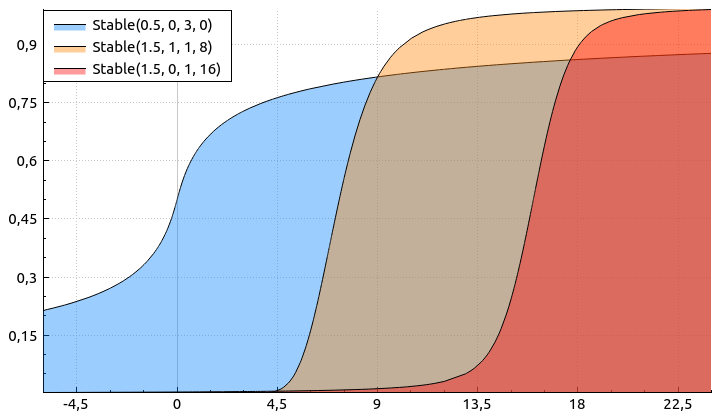
\includegraphics[width=\linewidth, right]{stable_cdf}
			\captionsetup{labelformat=empty}
		\end{minipage}
		\begin{minipage}{0.4\textwidth}
		\begin{tabular}{| r | l |}
			\hline
			Notation & $X \sim S_\alpha(\beta, \gamma, \mu)$ \\
			\hline
			Parameters & \pbox{\linewidth}{$\alpha \in (0, 2], \beta \in [-1, 1],$\\ $\gamma > 0, \mu \in \MR $} \\
			\hline
			Domain & \pbox{\linewidth}{$ x \in \MR$, if  $\beta \neq 1$, \\  $ x \in [\mu, \infty)  $, if  $\beta = 1$, $\alpha < 2$, \\ $ x \in (-\infty, \mu]  $, if  $\beta = -1$, $\alpha < 2$}  \\
			\hline
			$f(x)$ & Calculated numerically \\
			\hline
			$F(x)$ & Calculated numerically \\
			\hline
			$\ME[X]$ & \pbox{\linewidth}{$ \mu$ for $\alpha > 1$,\\ otherwise undefined} \\
			\hline
			$\Var(X)$ & $2 \gamma^2 1_{\{ \alpha = 2 \} } + \infty 1_{ \{ \alpha < 2 \} }  $ \\
			\hline
			Median & \pbox{\linewidth}{$\mu$ for $\beta = 0$,\\ otherwise searched numerically} \\
			\hline
			Mode & \pbox{\linewidth}{$\mu$, if $\beta = 0$ or $\alpha = 2$, \\  $\mu + \frac{\beta \gamma}{3}$, if $|\beta| = 1$ and $\alpha = \frac{1}{2}$, \\ otherwise searched numerically} \\
			\hline
			$\phi(t)$ & $ ...$ \\
			\hline
		\end{tabular}
	    \end{minipage}
	\end{figure}
	
	\paragraph{Calculation of p.d.f.}
	\paragraph{Calculation of c.d.f.}

\subsection{Cauchy distribution}
	Relation to Stable distribution:
	\[X \sim S_{1}(0, \gamma, \mu) \]
		\begin{figure}[!htb]\centering
		\begin{minipage}{0.55\textwidth}
			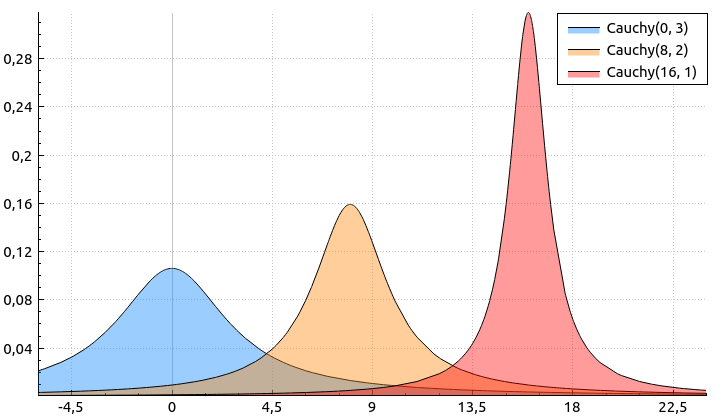
\includegraphics[width=\linewidth, right]{cauchy_pdf}
			\captionsetup{labelformat=empty}
			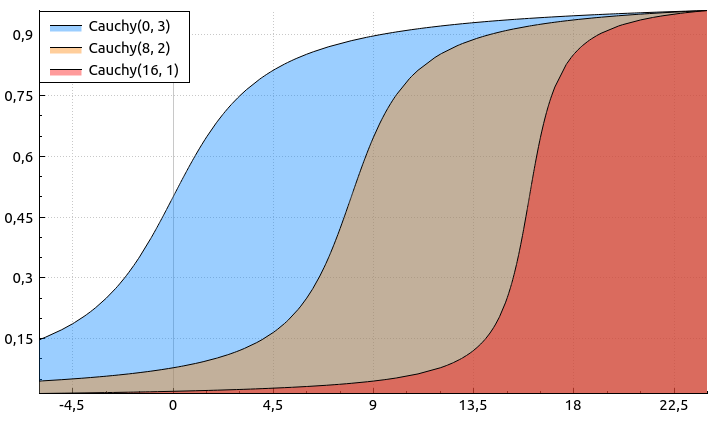
\includegraphics[width=\linewidth, right]{cauchy_cdf}
			\captionsetup{labelformat=empty}
		\end{minipage}
		\begin{minipage}{0.4\textwidth}
		\begin{tabular}{| r | l |}
			\hline
			Notation & $X \sim \operatorname{Cauchy}(\mu, \gamma)$ \\
			\hline
			Parameters & $\mu \in \MR, \gamma^2 > 0 $ \\
			\hline
			Domain & $x \in \MR$  \\
			\hline
			$f(x)$ & $ \frac{1}{ \pi \gamma \Big[ 1 + \big( \frac{x-\mu}{\gamma} \big)^2 \Big]  }  $ \\
			\hline
			$F(x)$ & $ \frac{1}{\pi} \operatorname{atan}\Big( \frac{x-\mu}{\gamma} \Big) + \frac{1}{2} $ \\
			\hline
			$\ME[X]$ & Undefined \\
			\hline
			$\Var(X)$ & $\infty $\\
			\hline
			Median & $\mu$ \\
			\hline
			Mode & $\mu$ \\
			\hline
			$\phi(t)$ & $ e^{i\mu t - \gamma |t|}  $ \\
			\hline
		\end{tabular}
	    \end{minipage}
	\end{figure}
	
	
\subsection{Levy distribution}
	Relation to Stable distribution:
	\[X \sim S_{\frac{1}{2}}(1, \gamma, \mu) \]

\subsection{Normal distribution}
Relation to Stable distribution:
\[X \sim S_{2}(\cdot, \sigma^2/2, \mu) \]

\begin{figure}[!htb]\centering
	\begin{minipage}{0.55\textwidth}
		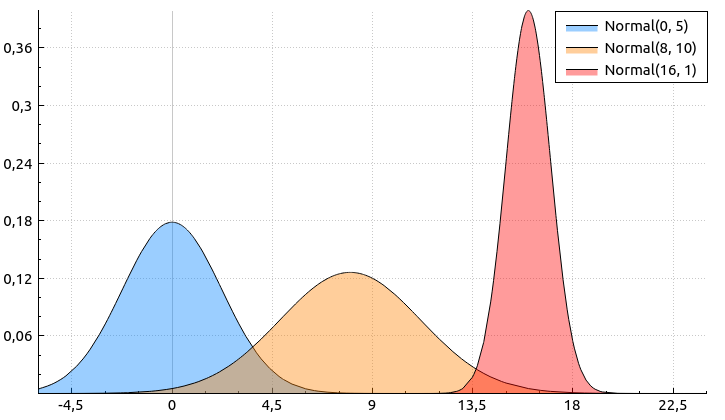
\includegraphics[width=\linewidth, right]{normal_pdf}
		\captionsetup{labelformat=empty}
		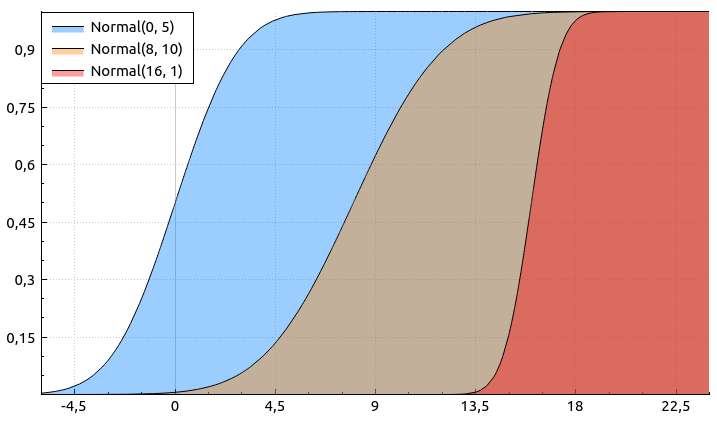
\includegraphics[width=\linewidth, right]{normal_cdf}
		\captionsetup{labelformat=empty}
	\end{minipage}
	\begin{minipage}{0.4\textwidth}
		\begin{tabular}{| r | l |}
			\hline
			Notation & $X \sim \mathcal{N}(\mu, \sigma^2)$ \\
			\hline
			Parameters & $\mu \in \MR, \sigma^2 > 0 $ \\
			\hline
			Domain & $x \in \MR$  \\
			\hline
			$f(x)$ & $ \frac{1}{\sqrt{2\sigma^2\pi}}e^{-\frac{(x-\mu)^2}{2\sigma^2}}  $ \\
			\hline
			$F(x)$ & $ \frac{1}{2} \operatorname{erfc}\Big( \frac{\mu-x}{\sqrt{2\sigma^2}} \Big) $ \\
			\hline
			$\ME[X]$ & $ \mu$ \\
			\hline
			$\Var(X)$ & $\sigma^2$\\
			\hline
			Median & $\mu$ \\
			\hline
			Mode & $\mu$ \\
			\hline
			$\phi(t)$ & $ e^{i\mu t - \frac{1}{2}\sigma^2t^2}  $ \\
			\hline
		\end{tabular}
	\end{minipage}
\end{figure}

\paragraph{Estimation of parameters}
\subparagraph{Frequentist inference.} Maximum-likelihood estimators for Normal distribution are very well-known:
\[
\hat{\mu} = \overline{X}_n \quad \text{and} \quad \hat{\sigma^2} = \frac{1}{n} \sum_{i=1}^{n} (X_i - \mu)^2.
\]
However, for unknown $\mu$ the value of $\hat{\sigma^2} \sim \frac{\sigma^2}{n}\chi^2_{n-1}$. Therefore, unbiased estimator in this case would be
\[
\widetilde{\sigma^2} = \frac{1}{n-1} \sum_{i=1}^{n} (X_i - \overline{X}_n)^2.
\]
Moreover, if one is interested in estimating scale $\sigma$ with known $\mu$, then maximum likelihood estimator is
\[
\hat{\sigma} = \sqrt{\hat{\sigma^2}} \sim \frac{\sigma}{\sqrt{n}} \chi_{n}
\]
and
\[
\ME[\hat{\sigma}] = \frac{\sigma}{\sqrt{n}} \sqrt{2} \frac{\Gamma((n+1)/2)}{\Gamma(n/2)}.
\]
Then unbiased estimator is
\[
\widetilde{\sigma} = \hat{\sigma} \sqrt{\frac{n}{2}} \frac{\Gamma(n/2)}{\Gamma((n+1)/2)}
\]

\subparagraph{Bayesian inference.}
...

\subsection{Holtsmark distribution}
	Relation to Stable distribution:
	\[X \sim S_{\frac{3}{2}}(0, \gamma, \mu) \]


\subsection{Landau distribution}
	Relation to Stable distribution:
	\[X \sim S_{1}(1, \gamma, \mu) \]
	
	
\pagebreak
\section{Weibull}

\begin{figure}[!htb]\centering
	\begin{minipage}{0.55\textwidth}
		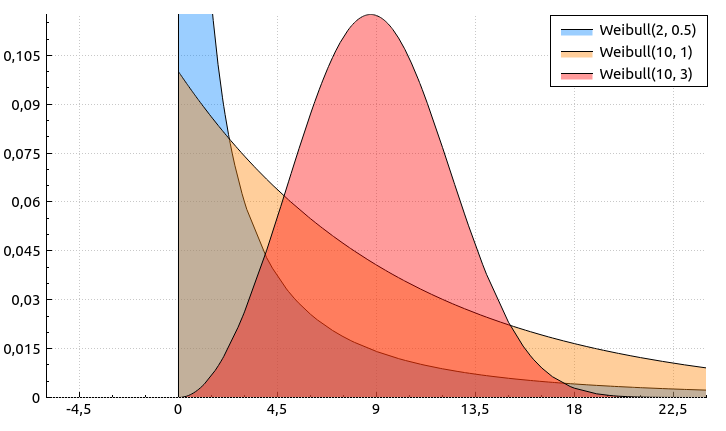
\includegraphics[width=\linewidth, right]{weibull_pdf}
		\captionsetup{labelformat=empty}
		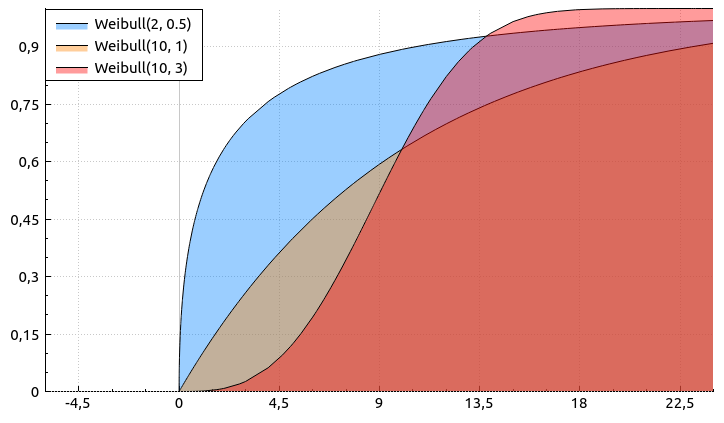
\includegraphics[width=\linewidth, right]{weibull_cdf}
		\captionsetup{labelformat=empty}
	\end{minipage}
	\begin{minipage}{0.4\textwidth}
		\begin{tabular}{| r | l |}
			\hline
			Notation & $X \sim \operatorname{Weibull}(\lambda, k)$ \\
			\hline
			Parameters & $\lambda, k > 0 $ \\
			\hline
			Domain & $x \in \MR^+$  \\
			\hline
			$f(x)$ & $ \frac{k}{\lambda}\big( \frac{x}{\lambda}\big)^{k-1} \exp(-(x/\lambda)^k)  $ \\
			\hline
			$F(x)$ & $ 1-\exp(-(x/\lambda)^k) $ \\
			\hline
			$\ME[X]$ & $ \lambda \Gamma(1+1/k)$ \\
			\hline
			$\Var(X)$ & $\lambda^2 \Gamma(1+2/k) - (\ME[X])^2$ \\
			\hline
			Median & $\lambda (\ln2)^{\frac{1}{k}}$ \\
			\hline
			Mode & $\lambda \big( 1-\frac{1}{k} \big)^{\frac{1}{k}}$ \\
			\hline
			$\phi(t)$ & Calculated numerically \\
			\hline
		\end{tabular}
	\end{minipage}
\end{figure}
\paragraph{Estimation of scale}.
\subparagraph{Frequentist inference.} Log-likelihood function:
\[
\ln \mathcal{L}(\lambda, k|X) = n (\ln k - \ln \lambda) + (k-1)\sum_{i=1}^{n}(\ln X_i - \ln \lambda) - \frac{1}{\lambda^k}\sum_{i=1}^{n} X_i^k.
\]
The derivative with respect to scale:
\[
\frac{\partial\ln \mathcal{L}(\lambda, k|X) }{\partial \lambda} = -\frac{n k}{\lambda} + \frac{k}{\lambda^{k+1}} \sum_{i=1}^{n} X_i^k=0.
\]
Therefore, maximum-likelihood estimation for $\lambda$ is
\[
\hat{\lambda} = \bigg(\frac{1}{n}\sum_{i=1}^{n}X_i^k\bigg)^{\frac{1}{k}}.
\]
\subparagraph{Bayesian inference.} Assume $k$ is known. Instead of estimating $\lambda$ we give an estimation for $\lambda^k$. Let's say that prior distribution of $\lambda^k$ is $\operatorname{Inv-\Gamma}(\alpha, \beta)$:
\[
h(\lambda^k) = \frac{\beta^\alpha}{\Gamma(\alpha)} \lambda^{-k(\alpha+1)} e^{-\beta / \lambda^k}.
\]
Posterior distribution then:
\[
f(\lambda^k| X) \propto \lambda^{-k(\alpha+1+n)} e^{-\frac{1}{\lambda^k} (\beta+\sum_{i=1}^{n}X_i^k)} \sim \operatorname{Inv-\Gamma}\bigg(\alpha+n, \beta+\sum_{i=1}^{n}X_i^k\bigg).
\]
Bayesian estimator:
\[
\ME[\lambda^k|X] = \frac{\beta+\sum_{i=1}^{n}X_i^k}{\alpha+n-1},
\]
MAP estimator:
\[
\lambda_{MAP}^k = \frac{\beta+\sum_{i=1}^{n}X_i^k}{\alpha+n+1}.
\]

	\pagebreak
	\part{Discrete univariate distributions}
	\section{Beta-binomial distribution}
	\begin{figure}[!htb]\centering
		\begin{minipage}{0.55\textwidth}
			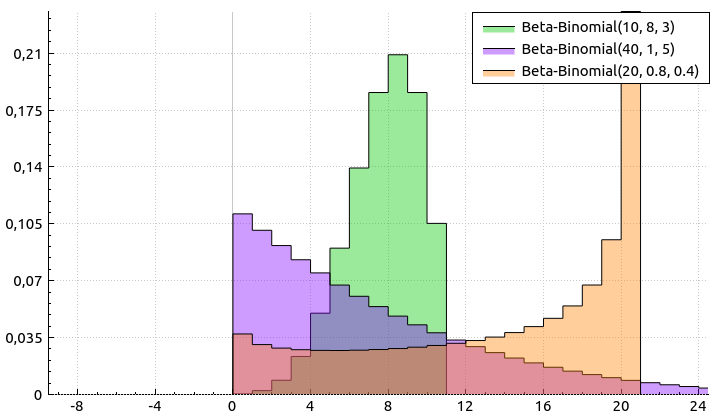
\includegraphics[width=\linewidth, right]{beta-binomial_pmf}
			\captionsetup{labelformat=empty}
			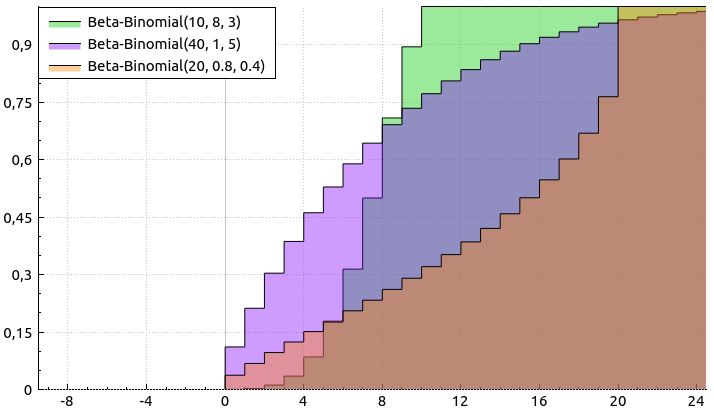
\includegraphics[width=\linewidth, right]{beta-binomial_cdf}
			\captionsetup{labelformat=empty}
		\end{minipage}
		\begin{minipage}{0.4\textwidth}
			\begin{tabular}{| r | l |}
				\hline
				Notation & $ X \sim \operatorname{BB}(n, \alpha, \beta) $ \\
				\hline
				Parameters & $ n \in \MN, \alpha, \beta > 0  $ \\
				\hline
				Domain & $ k \in \{0, \dots, n  \} $  \\
				\hline
				$\MP(X = k)$ & $\binom{n}{k} \frac{B(k+\alpha, n-k+\beta)}{B(\alpha, \beta)}  $ \\
				\hline
				$\MP(X \leq k)$ & Calculated numerically \\
				\hline
				$\ME[X]$ & $ n \frac{\alpha}{\alpha + \beta}$ \\
				\hline
				$\Var(X)$ & $\frac{n\alpha \beta (\alpha + \beta + n) }{(\alpha+\beta)^2(\alpha+\beta + 1)} $ \\
				\hline
				Median & Searched numerically \\
				\hline
				Mode & Searched numerically \\
				\hline
				$\phi(t)$ & Calculated numerically \\
				\hline
			\end{tabular}
		\end{minipage}
	\end{figure}

    Relation to other distributions: if $ p \sim \mathcal{B}(\alpha, \beta)$, then $\operatorname{Bin}(n, p) \sim \operatorname{BB}(n, \alpha, \beta)$.

	\pagebreak
	\section{Binomial distribution}
	\begin{figure}[!htb]\centering
		\begin{minipage}{0.55\textwidth}
			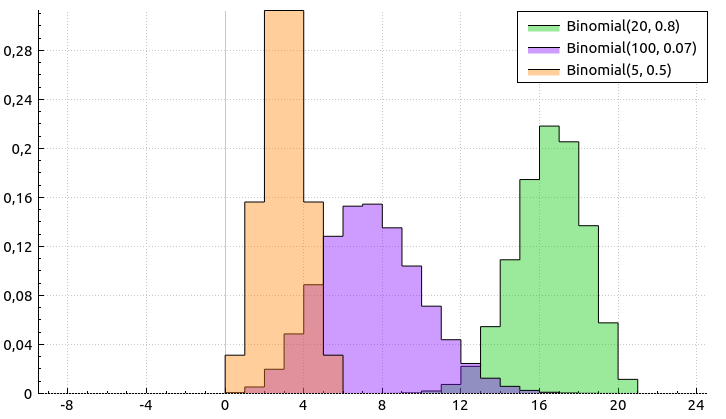
\includegraphics[width=\linewidth, right]{binomial_pmf}
			\captionsetup{labelformat=empty}
			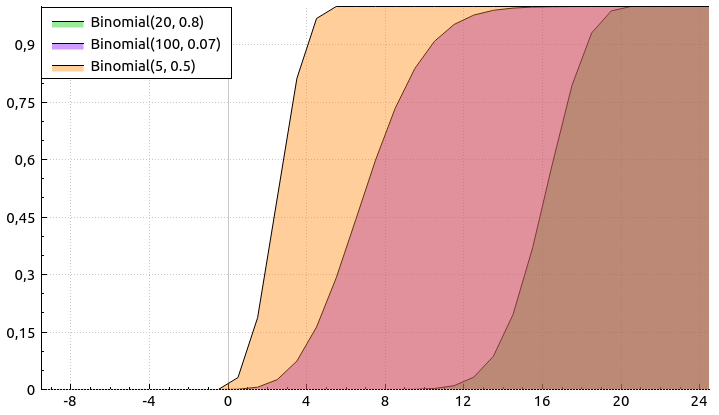
\includegraphics[width=\linewidth, right]{binomial_cdf}
			\captionsetup{labelformat=empty}
		\end{minipage}
		\begin{minipage}{0.4\textwidth}
			\begin{tabular}{| r | l |}
			\hline
			Notation & $ X \sim \operatorname{Bin}(n, p) $ \\
			\hline
			Parameters & $ n \in \MN, p \in [0, 1]  $ \\
			\hline
			Domain & $ k \in \{0, \dots, n  \} $  \\
			\hline
			$\MP(X = k)$ & $\binom{n}{k} p^k (1-p)^{n-k}  $ \\
			\hline
			$\MP(X \leq k)$ & $I_{1-p}(n-k, 1+k) $ \\
			\hline
			$\ME[X]$ & $ np$ \\
			\hline
			$\Var(X)$ & $np(1-p)$ \\
			\hline
			Median & $[np]$ \\
			\hline
			Mode & $[(n+1)p]$ \\
			\hline
			$\phi(t)$ & $ (1-p+pe^{it})^n  $ \\
			\hline
		\end{tabular}
		\end{minipage}
	\end{figure}
	
	\paragraph{Estimation of probability $p$ with known number $n$.}
	\subparagraph{Frequentist inference.} Log-likelihood function:
	\[
	\ln \mathcal{L}(p|X) \propto \sum_{i=1}^{k} \big(X_i \log p + (n-X_i) \log(1-p)\big)
	\]
	The derivative with respect to $p$ is:
	\[
	\frac{\partial \ln \mathcal{L}(p|X)}{\partial p} = \frac{\sum_{i=1}^k X_i}{p} - \frac{nk - \sum_{i=1}^{k}X_i}{1-p}.
	\]
	Therefore we reach the maximum value of log-likelihood if
	\[
	p = \frac{\overline X_k}{n}.
	\]
	
	\subparagraph{Bayesian inference.}
	We set prior Beta distribution $\mathcal{B}(\alpha, \beta)$:
	\[
	h(p) = \frac{p^{\alpha-1} (1-p)^{\beta - 1}}{B(\alpha, \beta)}.
	\]
	Then posterior is
	\[
	f(p|X) \propto p^{\alpha-1 + \sum_{i=1}^k X_i} (1-p)^{\beta - 1 + \sum_{i=1}^k (n - X_i)} \sim \mathcal{B}\bigg(\alpha + \sum_{i=1}^k X_i, \beta + nk - \sum_{i=1}^k X_i\bigg).
	\]
	Thus Bayesian estimator is
	\[ \mathbb{E}[p|X] = \frac{\alpha + \sum_{i=1}^k X_i}{\alpha + \beta + nk} \]
	and MAP estimator is
	\[ p_{MAP} = \frac{\alpha + \sum_{i=1}^k X_i - 1}{\alpha + \beta + nk - 2}. \]
	Also, Minimax estimator is equal to Bayes estimator if $\alpha = \beta = \frac{1}{2}\sqrt{n}$.
	
	
	\subsection{Bernoulli}
	Notation:
	\[ X \sim \operatorname{Bernoulli}(p). \]
	Relation to Binomial distribution: \[X \sim \operatorname{Bin}(1, p). \]
	
	\pagebreak
	\section{Hypergeometric distribution}
		\begin{figure}[!htb]\centering
			\begin{minipage}{0.55\textwidth}
				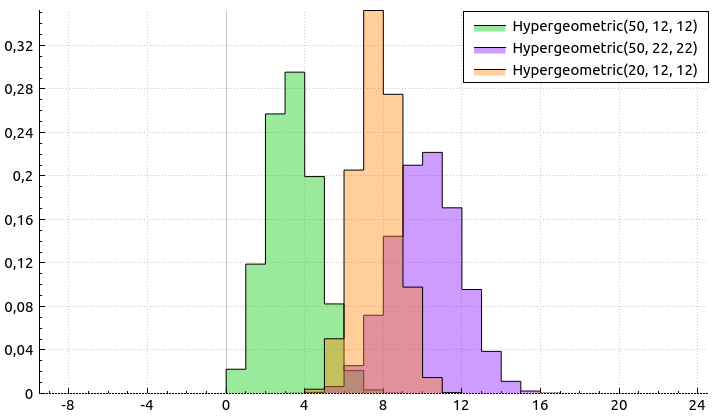
\includegraphics[width=\linewidth, right]{hypergeometric_pmf}
				\captionsetup{labelformat=empty}
				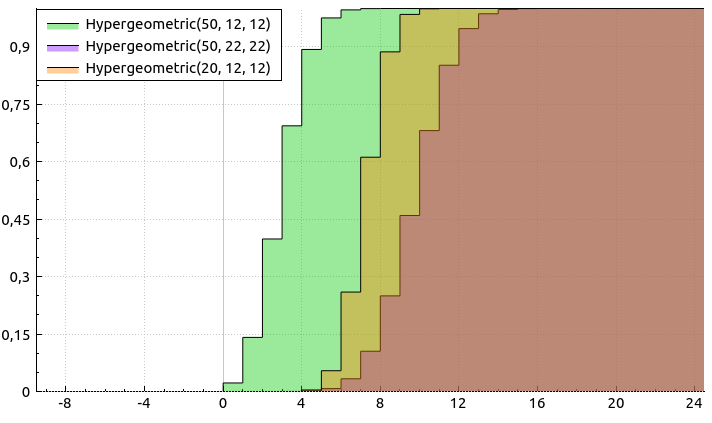
\includegraphics[width=\linewidth, right]{hypergeometric_cdf}
				\captionsetup{labelformat=empty}
			\end{minipage}
			\begin{minipage}{0.4\textwidth}
				\begin{tabular}{| r | l |}
					\hline
					Notation & $ X \sim \operatorname{HG}(N, K, n) $ \\
					\hline
					Parameters & 
					\pbox{\linewidth}{$ N \in \MN, K \in \{1, 2, \dotsm, N  \},$ \\ $n \in \{1, 2, \dotsm, N  \}$} \\
					\hline
					Domain & $ \max(0, n+K-N) \leq k \leq \min(n, K) $  \\
					\hline
					$\MP(X = k)$ & $ \frac{\binom{K}{k}\binom{N-K}{n-k}  }{\binom{N}{n}}   $ \\
					\hline
					$\MP(X \leq k)$ & Calculated numerically \\
					\hline
					$\ME[X]$ & $ \frac{nK}{N}$ \\
					\hline
					$\Var(X)$ & $ \frac{nK(N-K)(N-n)}{N^2(N-1)} $ \\
					\hline
					Median & Searched numerically \\
					\hline
					Mode & $ \Big\lfloor  \frac{(n+1)(K+1)}{N+2} \Big\rfloor  $ \\
					\hline
					$\phi(t)$ & Calculated numerically \\
					\hline
				\end{tabular}
			\end{minipage}
		\end{figure}
		
	\paragraph{Estimation of number of target members of population K.}
	\subparagraph{Bayesian inference.}
	Let prior distribution of $K$ be Beta-Binomial distribution $BB(N, \alpha, \beta)$:
	\[
	h(K) = \binom{N}{K} \frac{B(K + \alpha, N - K + \beta)}{B(\alpha, \beta)}.
	\]
	Then for one sample $X$:
    \[
    K - X \sim BB\big(N - n, \alpha + X, \beta + nk - X \big)
    \]
    and therefore
    \[ 
    \mathbb{E}[K|X] = X + (N - n) \frac{\alpha}{\alpha + \beta}.
    \]
    However, RandLib doesn't support Bayesian fitting for Hypergeometric distribution yet.
    
		
	\pagebreak
	\section{Negative-Binomial (Polya) distribution}
	\begin{figure}[!htb]\centering
		\begin{minipage}{0.55\textwidth}
			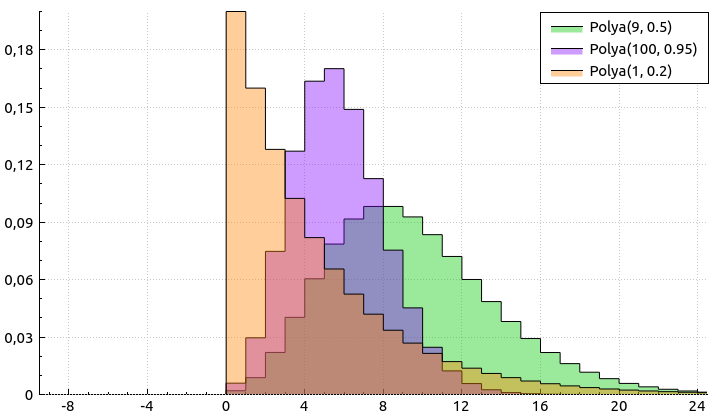
\includegraphics[width=\linewidth, right]{negative-binomial_pmf}
			\captionsetup{labelformat=empty}
			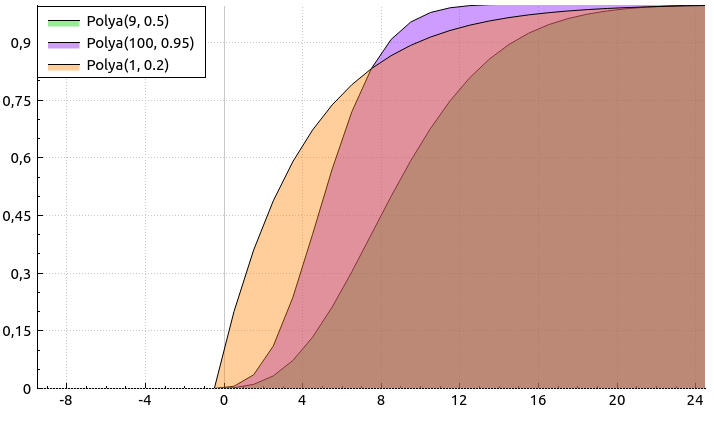
\includegraphics[width=\linewidth, right]{negative-binomial_cdf}
			\captionsetup{labelformat=empty}
		\end{minipage}
		\begin{minipage}{0.4\textwidth}
			\begin{tabular}{| r | l |}
				\hline
				Notation & $ X \sim \operatorname{NB}(r, p) $\\
				\hline
				Parameters & $r > 0$, $p \in (0, 1)$ \\
				\hline
				Domain & $ k \in \MN_0 $  \\
				\hline
				$\MP(X = k)$ & $  \binom{k+r-1}{k} p^r (1-p)^k   $ \\
				\hline
				$\MP(X \leq k)$ & $I_p(r, k+1)$ \\
				\hline
				$\ME[X]$ & $ \frac{1-p}{p}r$ \\
				\hline
				$\Var(X)$ & $ \frac{1-p}{p^2}r $ \\
				\hline
				Median & Searched numerically \\
				\hline
				Mode & $ \max\Big(\Big\lfloor  \frac{(r-1)(1-p)}{p} \Big\rfloor, 0\Big)  $ \\
				\hline
				$\phi(t)$ & $\Big( \frac{p}{1-(1-p)e^{it}} \Big)^r$  \\
				\hline
			\end{tabular}
		\end{minipage}
	\end{figure}
	Relation to other distributions: if $\lambda \sim \operatorname{Gamma}\big(r, \frac{p}{1-p}\big)$, then $\operatorname{Po}(\lambda) \sim \operatorname{NB}(r, p)$.
	
	\subsection{Geometric distribution}
	Notation:
	\[
	X \sim \operatorname{Geometric}(p).
	\]
	Relation to Negative-Binomial distribution:
	\[
	X \sim \operatorname{NB}(1, p).
	\]
	\subsection{Pascal distribution}
	Notation:
	\[
	X \sim \operatorname{Pascal}(r, p).
	\]
	The only difference with Negative-Binomial distribution is that for Pascal distribution shape $r$ is an integer.
	
	\pagebreak
	\section{Poisson distribution}
		\begin{figure}[!htb]\centering
			\begin{minipage}{0.55\textwidth}
				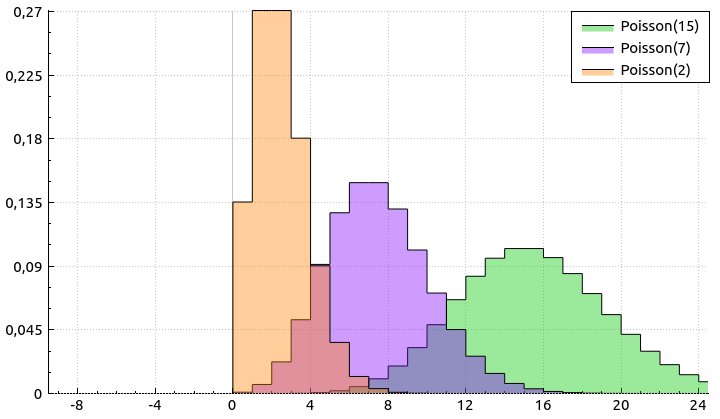
\includegraphics[width=\linewidth, right]{poisson_pmf}
				\captionsetup{labelformat=empty}
				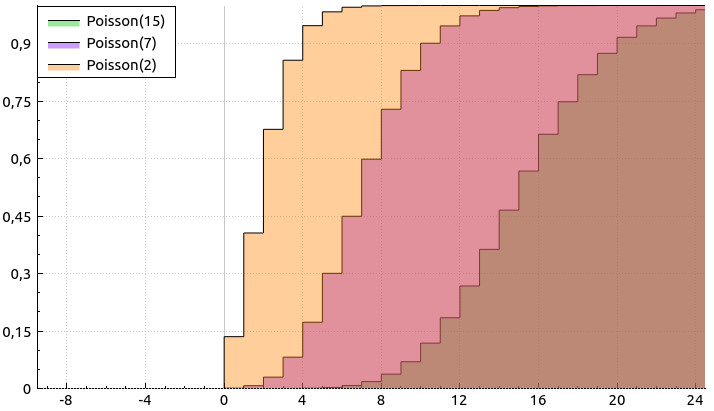
\includegraphics[width=\linewidth, right]{poisson_cdf}
				\captionsetup{labelformat=empty}
			\end{minipage}
			\begin{minipage}{0.4\textwidth}
				\begin{tabular}{| r | l |}
					\hline
					Notation & $ X \sim \operatorname{Po}(\lambda) $ \\
					\hline
					Parameters & $\lambda > 0$ \\
					\hline
					Domain & $ k \in \MN_0 $  \\
					\hline
					$\MP(X = k)$ & $\frac{\lambda^k e^{-\lambda}}{k!}$ \\
					\hline
					$\MP(X \leq k)$ & $Q(k+1, \lambda)$ \\
					\hline
					$\ME[X]$ & $ \lambda$ \\
					\hline
					$\Var(X)$ & $\lambda$ \\
					\hline
					Median & $\sim \max\big([\lambda + \frac{1}{3} - \frac{0.02}{\lambda}], 0\big) $ \\
					\hline
					Mode & $[\lambda]$ \\
					\hline
					$\phi(t)$ & $ \exp \{ \lambda(e^{it}-1) \}  $ \\
					\hline
				\end{tabular}
			\end{minipage}
		\end{figure}
	
	\paragraph{Estimation of rate.}
	\subparagraph{Frequentist inference.}
	Log-likelihood function:
	\[ \ln \mathcal{L}(\lambda | X) \propto -\lambda n + \sum_{i=1}^{n}X_i \log \lambda. \]
	Setting the derivative w.r.t. rate to $0$ we get the optimal value:
	\[ \lambda = \overline{X}_n. \]
	\subparagraph{Bayesian inference.}
	Let set prior distribution of $\lambda \sim \Gamma(\alpha, \beta)$:
	\[
	h(\lambda) = \frac{\beta^\alpha}{\Gamma(\alpha)} \lambda^{\alpha-1}e^{-\beta \lambda}.
	\]
	Posterior distribution:
	\[
	f(\lambda|X) \propto e^{-\lambda (\beta + n)}  \lambda^{\alpha - 1 + \sum_{i=1}^{n}X_i} \sim \Gamma(\alpha + \sum_{i=1}^{n}X_i, \beta + n).
	\]
	Therefore, Bayesian estimator:
	\[
	\mathbb{E}[\lambda|X] = \frac{\alpha + \sum_{i=1}^{n}X_i}{\beta + n}.
	\]
	And MAP estimator:
	\[
	\lambda_{MAP} = \max \bigg( \frac{\alpha + \sum_{i=1}^{n}X_i - 1}{\beta + n}, 0 \bigg).
	\]
	
	\paragraph{Exponential family parameterization}
	Logarithm of probability mass function:
	\[
	\log \MP(X = x) = x \log \lambda - \lambda - \log(x!).
	\]
	Therefore, sufficient statistics $T(x) = x$, natural parameter $\theta = \log \lambda$, log-normalizer $F(\theta) = \exp(\theta)$, carrier measure $k(x) = \log(x!)$. We conclude that adjusted cross-entropy is
	\[
	\begin{aligned}
	H_F(\theta_q \| \theta_p) &= F(\theta_q) - \langle \theta_q, \nabla F(\theta_p) \rangle \\
	&= \exp(\theta_q) - \theta_q \exp(\theta_p).
	\end{aligned}
	\]
	Adjusted entropy is
	\[
	H_F(\theta) = \exp(\theta) (1 - \theta) = \lambda (1 - \log \lambda).
	\]
	And Kullback-Leibler divergence:
	\[
	\begin{aligned}
	\operatorname{KL}(p \| q) &= H_F(\theta_q \| \theta_p) - H_F(\theta_p) \\
	&= \lambda_q -  \lambda_p \bigg(1 + \log \bigg(\frac{\lambda_p}{\lambda_q}\bigg)\bigg).
	\end{aligned}
	\]
	
	
	\pagebreak
	\section{Skellam distribution}
	
	\begin{figure}[!htb]\centering
		\begin{minipage}{0.55\textwidth}
			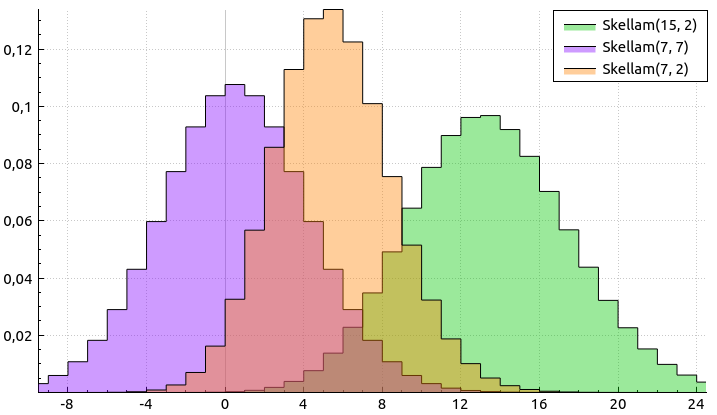
\includegraphics[width=\linewidth, right]{skellam_pmf}
			\captionsetup{labelformat=empty}
			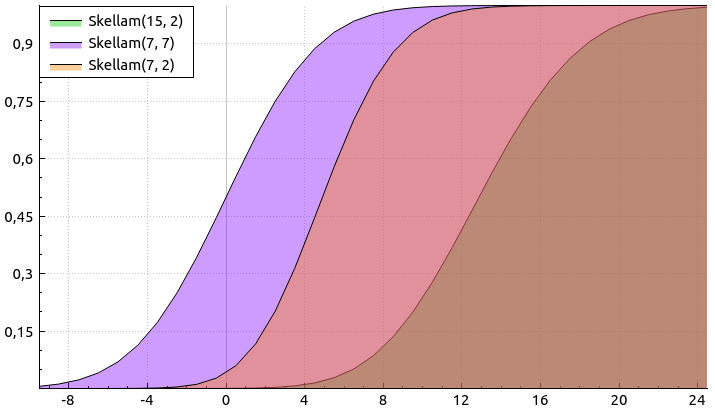
\includegraphics[width=\linewidth, right]{skellam_cdf}
			\captionsetup{labelformat=empty}
		\end{minipage}
		\begin{minipage}{0.4\textwidth}
			\begin{tabular}{| r | l |}
				\hline
				Notation & $ X \sim \operatorname{Skellam}(\mu_1, \mu_2) $ \\
				\hline
				Parameters & $\mu_1, \mu_2 > 0$ \\
				\hline
				Domain & $ k \in \MZ $  \\
				\hline
				$\MP(X = k)$. & $e^{-(\mu_1 + \mu_2)} \Big( \frac{\mu_1}{\mu_2} \Big)^{\frac{k}{2}} I_k(2\sqrt{\mu_1\mu_2}) $ \\
				\hline
				$\MP(X \leq k)$ & \pbox{\linewidth}{$\operatorname{MarcumP}_{k+1}(\mu_2, \mu_1)$, $k \geq 0$ \\ $\operatorname{MarcumQ}_{-k}(\mu_1, \mu_2)$, $k < 0$ } \\
				\hline
				$\ME[X]$ & $ \mu_1-\mu_2$ \\
				\hline
				$\Var(X)$ & $\mu_1+\mu_2$ \\
				\hline
				Median & Searched numerically \\
				\hline
				Mode & $[ \mu_1-\mu_2] $ \\
				\hline
				$\phi(t)$ & $ \exp \{ \mu_1(e^{it}-1) - \mu_2(e^{it}-1) \}  $ \\
				\hline
			\end{tabular}
		\end{minipage}
	\end{figure}
	Relation to other distributions: if $Y \sim \operatorname{Po}(\mu_1)$ and $Z \sim \operatorname{Po}(\mu_2)$, then
	\[
	Y - Z \sim \operatorname{Skellam}(\mu_1, \mu_2).
	\]
	
	\pagebreak
	\section{Uniform discrete distribution}
	\begin{figure}[!htb]\centering
		\begin{minipage}{0.55\textwidth}
			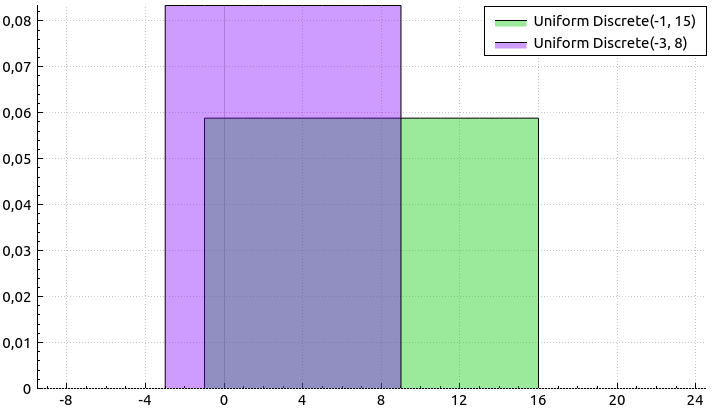
\includegraphics[width=\linewidth, right]{uniform_discrete_pmf}
			\captionsetup{labelformat=empty}
			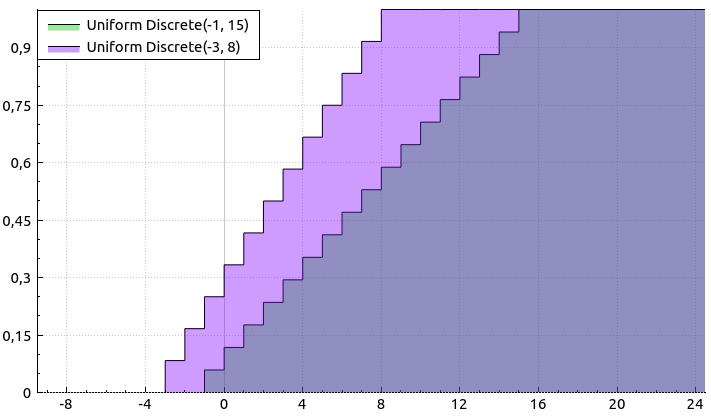
\includegraphics[width=\linewidth, right]{uniform_discrete_cdf}
			\captionsetup{labelformat=empty}
		\end{minipage}
		\begin{minipage}{0.4\textwidth}
			\begin{tabular}{| r | l |}
				\hline
				Notation & $ X \sim \mathcal{U}\{a, \dots, b\} $ \\
				\hline
				Parameters & $a, b \in \MR, a \leq b$ \\
				\hline
				Domain & $ k \in \{a, \dots, b\} $  \\
				\hline
				$\MP(X = k)$ & $\frac{1}{n} $, where $n=b-a+1$. \\
				\hline
				$\MP(X \leq k)$ & $\frac{k-a+1}{n}$ \\
				\hline
				$\ME[X]$ & $ \frac{a+b}{2} $ \\
				\hline
				$\Var(X)$ & $ \frac{(n-1)(n+1)}{12}$\\
				\hline
				Median & $\frac{a+b}{2}$ \\
				\hline
				Mode & Any value between $a$ and $b$ \\
				\hline
				$\phi(t)$ & $\frac{\cos(at)-\cos((b+1)t)+i(\sin(at)-\sin((b+1)t))}{n(1-\cos(t)-i\sin(t))}$ \\
				\hline
			\end{tabular}
		\end{minipage}
	\end{figure}
	
	Relation to other distributions: if $X \sim BB(n, 1, 1)$, then $X \sim \mathcal{U}\{0, \dots, n\}$.
	
	\pagebreak
	\section{Yule distribution}
	\begin{figure}[!htb]\centering
		\begin{minipage}{0.55\textwidth}
			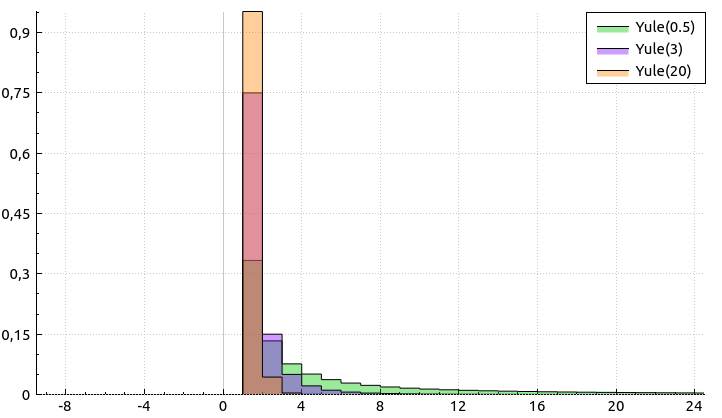
\includegraphics[width=\linewidth, right]{yule_pmf}
			\captionsetup{labelformat=empty}
			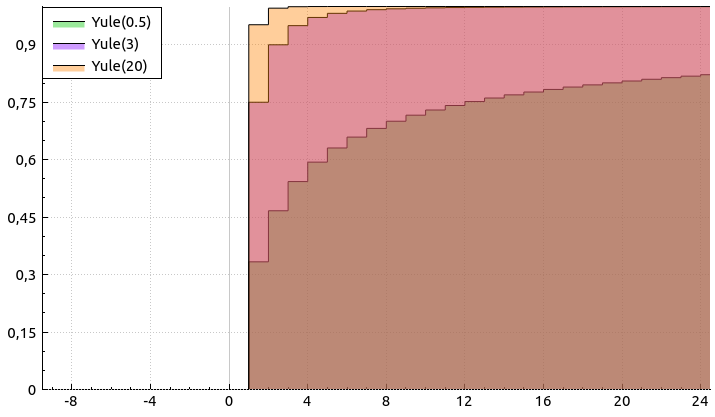
\includegraphics[width=\linewidth, right]{yule_cdf}
			\captionsetup{labelformat=empty}
		\end{minipage}
		\begin{minipage}{0.4\textwidth}
			\begin{tabular}{| r | l |}
				\hline
				Notation & $ X \sim \operatorname{Yule}(\rho) $ \\
				\hline
				Parameters & $\rho \in \MR^+$ \\
				\hline
				Domain & $ k \in \MN $  \\
				\hline
				$\MP(X = k)$ & $\rho \frac{ \Gamma(1+\rho) (k-1)! } {\Gamma(k+\rho+1)} $ \\
				\hline
				$\MP(X \leq k)$ & $1-k \frac{ \Gamma(1+\rho) (k-1)! } {\Gamma(k+\rho+1)} $ \\
				\hline
				$\ME[X]$ & \pbox{\linewidth}{$ \frac{\rho}{\rho - 1}$, $\rho > 1$ \\ $\infty$, otherwise } \\
				\hline
				$\Var(X)$ & \pbox{\linewidth}{$ \frac{\rho^2}{(\rho - 1)^2(\rho-2)}$, $\rho > 2$ \\ $\infty$, otherwise } \\
				\hline
				Median & Searched numerically \\
				\hline
				Mode & $1 $ \\
				\hline
				$\phi(t)$ & Calculated numerically \\
				\hline
			\end{tabular}
		\end{minipage}
	\end{figure}
	Relation to other distributions: if $X \sim \operatorname{Pareto}(\alpha, 1)$, then $\operatorname{Geometric}(1/X) \sim \operatorname{Yule}(\alpha)$.
	
	\pagebreak
	\section{Zeta distribution}
		\begin{figure}[!htb]\centering
			\begin{minipage}{0.55\textwidth}
				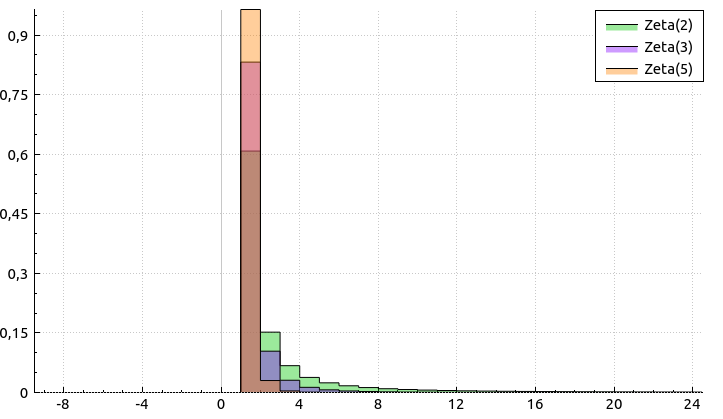
\includegraphics[width=\linewidth, right]{zeta_pmf}
				\captionsetup{labelformat=empty}
				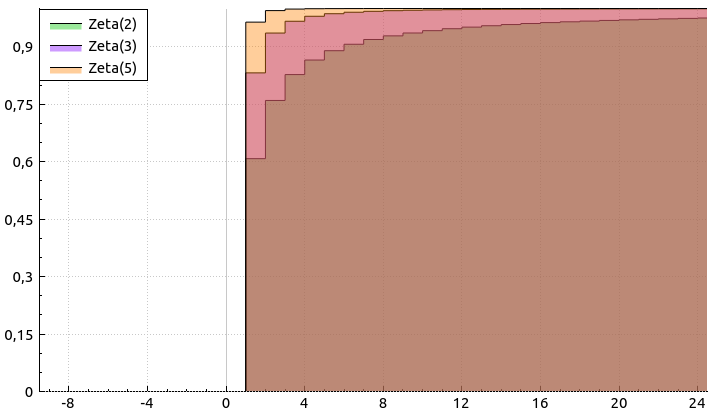
\includegraphics[width=\linewidth, right]{zeta_cdf}
				\captionsetup{labelformat=empty}
			\end{minipage}
			\begin{minipage}{0.4\textwidth}
				\begin{tabular}{| r | l |}
					\hline
					Notation & $ X \sim \operatorname{Zeta}(s) $ \\
					\hline
					Parameters & $s > 1$ \\
					\hline
					Domain & $ k \in \MN $  \\
					\hline
					$\MP(X = k)$ & $ \frac{1}{\zeta(s) k^s} $ \\
					\hline
					$\MP(X \leq k)$ & $ \frac{H(s, k)}{\zeta(s)} $ \\
					\hline
					$\ME[X]$ & \pbox{\linewidth}{$ \frac{\zeta(s-1)}{\zeta(s)}$, $s > 2$ \\ $\infty$, otherwise } \\
					\hline
					$\Var(X)$ & \pbox{\linewidth}{$ \frac{\zeta(s-2)}{\zeta(s)} - (\ME[X])^2$, $\rho > 3$ \\ $\infty$, otherwise } \\
					\hline
					Median & Searched numerically \\
					\hline
					Mode & $1 $ \\
					\hline
					$\phi(t)$ & Calculated numerically \\
					\hline
				\end{tabular}
			\end{minipage}
		\end{figure}
		
	\pagebreak
	\section{Zipf distribution}
	
	\pagebreak
	\part{Bivariate distributions}
	\section{Bivariate Normal distribution}
	\section{Normal-Inverse-Gamma distribution}
	\section{Trinomial distribution}
	
	\pagebreak
	\part{Circular distributions}
	\section{von Mises distribution}
	\section{Wrapped Exponential distribution}
	
	\pagebreak
	\part{Singular distributions}
	\section{Cantor distribution}
	
\end{document}
